%%%%%% NOTE NOTE NOTE %%%%%%%
% This manuscript has all lines wrapped to 120 characters. Save yourself some trouble and set your editor to be that
% wide! <3 Nolan



	% FIRST OF ALL:
% If you are using X-based Emacs to read this file, please switch on
% Syntax Highlighting by typing:
%    ALT-X  font-lock-mode   (or META-X on X-Terminals)
%
% That should make these comments nice and red so they can be easily
% distinguished from the actual code.
% =======================================================================

% This is a template for  Masters' Theses at WPI.
% It complies (more or less) to the standards given by the Library
% (as of February 1999)
%
% Feel free to use this file, but I give no guarantee for its compliance
% to standards (meaning I won't pay for the paper if the library rejects it :))
%
%
% The lengths (textheight, width etc.) are fine-tuned for ps1, ps2, and ps3,
% but seem to be somewhat dependent on the machine you are using to compile,
% the date, time, moon phase, the weather, and other quantum effects.
% You may have to change \oddsidemargin a little, but it's about 98% correct.
%
% Also, the spacing is correct (doublespacing with footnotes correctly
% singlespaced). Curiously, the font size is not specified in the
% regulations. So feel free to change it, but the majority of theses
% that I have seen is written in 12 point font.
%
% As for the inclusion of graphics, I recommend the methods specified
% in ``latexguide.ps'' off the CS-GSO Website. You can use other
% methods including copy and paste with a photocopier, but I think
% using the graphicx package is the easiest.
%
% Have fun and good luck with the thesis.
%
%
%  Andreas Koeller (koeller@wpi.edu)
%
%
%

% The preamble
%
%
% 12 point font, and your thesis is a ``report'' to LaTeX
\documentclass[12pt]{report}

% this enables correct linespacing and graphics inclusion via
%``\includegraphics''
\usepackage[english]{babel}
\usepackage{acro}
\usepackage{setspace}
\usepackage{graphicx}
%\usepackage[]{algorithm2e}
%\usepackage{algpseudocode}
\usepackage{algpseudocode,algorithm,algorithmicx}
\usepackage{amsmath, amsfonts, amssymb, amsthm}
\usepackage{bm}
\usepackage{todonotes}
\usepackage{float}
\usepackage[bottom]{footmisc}
\usepackage[utf8]{inputenc}


% Environments

\newtheorem{theorem}{Theorem}[section]
\newtheorem{corollary}{Corollary}[theorem]
\newtheorem{lemma}[theorem]{Lemma}
\newtheorem{assumption}[theorem]{Assumption}
\newtheorem{problem}[theorem]{Problem}
\newtheorem{proposition}[theorem]{proposition}
\newtheorem{definition}[theorem]{Definition}
\newtheorem{remark}[theorem]{Remark}

% Link acronyms (uses acro package), definitions and shortcuts.
% Planning and Trajectory Generation Acronyms

\DeclareAcronym{DRA}{
    short = DRA,
    long = Deterministic Raban Automaton ,
    class = abbrev
}

\DeclareAcronym{LTL}{
    short = LTL,
    long = Linear Temporal Logic ,
    class = abbrev,
    short-indefinite = an
}

\DeclareAcronym{MDP}{
    short = MDP,
    long = Markov Decision Process ,
    class = abbrev,
    short-indefinite = an,
}

\DeclareAcronym{SGA}{
    short = SGA,
    long = Stochastic Gradient Ascent ,
    class = abbrev,
    short-indefinite = an,
}

\DeclareAcronym{MLE}{
    short = MLE,
    long = Maximum Likelihood Estimate ,
    class = abbrev,
    short-indefinite = an,
}


\DeclareAcronym{GGK}{
    short = GGK,
    long = Geodesic Gaussian Kernel ,
    class = abbrev,
}

\DeclareAcronym{OGK}{
    short = OGK,
    long = Ordinary Gaussian Kernel ,
    class = abbrev,
    short-indefinite = an,
    long-indefinite = an
}

\DeclareAcronym{KLD}{
    short = KL-divergence,
    long =  Kullback-Leibler divergence ,
    class = abbrev,
}

\DeclareAcronym{ED}{
    short = \ensuremath{\text{ED}},
    long =  Euclidian Distance ,
    class = abbrev,
    short-indefinite = an,
}

\DeclareAcronym{SP}{
    short = \ensuremath{\text{SP}},
    long =  Shortest Path ,
    class = abbrev,
    short-indefinite = an,
}

\DeclareAcronym{RL}{
    short = RL,
    long =  Reinforcement Learning,
    class = abbrev,
    short-indefinite = an,
}

\DeclareAcronym{EM}{
	short = EM,
	long = Expectation Maximization,
}

\DeclareAcronym{HiPMDP}{short = HiP-MDP , long = Hidden Parameter Markov Decision Process }
\DeclareAcronym{MOMDP}{short = MOMDP , long = Mixed-Observability MDP, short-indefinite=an }
\DeclareAcronym{POMDP}{short = POMDP , long = Partially-Observable MDP }
\DeclareAcronym{pgpe}{short = PGPE , long = policy gradients with parameter-based exploration }


%%%%%%%%%%%%%%%%%%%%%%%%%%%%%%%%%%%%%%%%%%%%%%%%%%%%%%%%%%%%%%%%%%%%%%%%%%%%%%%%
\newif\ifuseboldmathops
\newif\ifuseittextabbrevs
\useboldmathopstrue   % comment out to use mathbb
%\useittextabbrevstrue % comment out to use non-italic text abbrevs like e.g.
%%%%%%%%%%%%%%%%%%%%%%%%%%%%%%%%%%%%%%%%%%%%%%%%%%%%%%%%%%%%%%%%%%%%%%%%%%%%%%%%

%%%  	Imported from WPI-template 	%%%
% Define \brk as a command for leaving a little vertical space. Makes
% the titlepage easier to read - normally, this is NOT GOOD LATEX
% STYLE!!!
%
\newcommand{\brk}{\vspace*{0.18in}}

%First, we want to make our life easier and define a ``TAB'' command.
\newcommand{\T}{\hspace*{5mm}}

%%% 	Math operators		        %%%
\ifuseboldmathops
    \newcommand{\vect}[1]{\boldsymbol{\mathbf{#1}}}
\else
    \newcommand{\vect}[1]{\boldsymbol{\mathbb{#1}}}
\fi

\newcommand{\estimate}[1]{\ensuremath{\hat{#1}}}
\newcommand{\optimal}[1]{\ensuremath{#1^*}}
\newcommand{\error}[1]{\ensuremath{\tilde{#1}}}
\newcommand{\OneNorm}[1]{\ensuremath{\left|#1\right|_1}}


% text abbrevs
\ifuseittextabbrevs
\newcommand{\cf}{{\it cf.}}
\newcommand{\eg}{{\it e.g.}}
\newcommand{\ie}{{\it i.e.}}
\newcommand{\etc}{{\it etc.}}
\newcommand{\etal}{{et~al.}}
\else
\newcommand{\cf}{cf.}
\newcommand{\eg}{e.g.}
\newcommand{\ie}{i.e.}
\newcommand{\etc}{etc.}
\newcommand{\etal}{et~al.}
\fi

% standard math sets
\ifuseboldmathops
%\newcommand{\reals}{{\mbox{\bf R}}}
\newcommand{\reals}{\mathbf{R}}
\newcommand{\integers}{\mathbf{Z}}
\newcommand{\complex}{\mathbf{C}}
\newcommand{\symm}{\mathbf{S}}  % symmetric matrices
\else
\newcommand{\reals}{\mathbb{R}}
\newcommand{\integers}{\mathbb{Z}}
\newcommand{\complex}{\mathbb{C}}
\newcommand{\symm}{\mathbb{S}}  % symmetric matrices
\fi

% control theory sets
\ifuseboldmathops
\newcommand{\HH}{\mathbf{H}}
\newcommand{\LL}{\mathbf{L}}
\else
\newcommand{\HH}{\mathbb{H}}
\newcommand{\LL}{\mathbb{L}}
\fi

% probability operators
\ifuseboldmathops
\newcommand{\Expect}{\mathop{\bf E{}}\nolimits}
\newcommand{\Prob}{\mathop{\bf P{}}\nolimits}
\else
\newcommand{\Expect}{\mathop{\mathbb{E}{}}\nolimits}
\newcommand{\Prob}{\mathop{\mathbb{P}{}}\nolimits}
\fi

% convex operators
\ifuseboldmathops
\renewcommand{\Re}{\mathop{\bf Re}}
\renewcommand{\Im}{\mathop{\bf Im}}

\newcommand{\prox}{\mathop{\bf prox}} % proximal operator
\newcommand{\dom}{\mathop{\bf dom}}   % domain
\newcommand{\aff}{\mathop{\bf aff}}   % affine hull
\newcommand{\cl}{\mathop{\bf cl}}     % closure
\newcommand{\intr}{\mathop{\bf int}}  % interior
\newcommand{\Co}{\mathop{\bf Co}}     % convex hull
\newcommand{\relint}{\mathop{\bf rel int}} % relative interior
\newcommand{\bd}{\mathop{\bf bd}}     % boundary

\newcommand{\Tr}{\mathop{\bf Tr}}
\newcommand{\diag}{\mathop{\bf diag}}
\else
\renewcommand{\Re}{\mathop{\mathrm{Re}}}
\renewcommand{\Im}{\mathop{\mathrm{Im}}}

\newcommand{\prox}{\mathop{\mathrm{prox}}} % proximal operator
\newcommand{\dom}{\mathop{\mathrm{dom}}}   % domain
\newcommand{\aff}{\mathop{\mathrm{aff}}}   % affine hull
\newcommand{\cl}{\mathop{\mathrm{cl}}}     % closure
\newcommand{\intr}{\mathop{\mathrm{int}}}  % interior
\newcommand{\Co}{\mathop{\mathrm{Co}}}     % convex hull
\newcommand{\relint}{\mathop{\mathrm{rel int}}} % relative interior
\newcommand{\bd}{\mathop{\mathrm{bd}}}     % boundary

\newcommand{\Tr}{\mathop{\mathrm{Tr}}}     % trace
\newcommand{\diag}{\mathop{\mathrm{diag}}} % diagonal matrix
\fi

% useful non-bold operators
\newcommand{\eqbydef}{\mathrel{\stackrel{\Delta}{=}}}
\newcommand{\eqbyset}{\mathrel{\stackrel{\mathrm{set}}{=}}}
\newcommand{\argmax}{\mathop{\mathrm{argmax}}}
\newcommand{\argmin}{\mathop{\mathrm{argmin}}}

% lin alg stuff
\newcommand{\Span}{\mathop{\mathrm{span}}}
\newcommand{\Range}{\mathop{\mathrm{range}}}
\newcommand{\Null}{\mathop{\mathrm{null}}}
\newcommand{\rank}{\mathop{\mathrm{rank}}}

\newcommand{\ones}{\mathbf 1}
\newcommand{\lambdamax}{{\lambda_{\rm max}}}
\newcommand{\lambdamin}{{\lambda_{\rm min}}}
\newcommand{\sigmamax}{{\sigma_{\rm max}}}
\newcommand{\sigmamin}{{\sigma_{\rm min}}}

% linear temporal logic
% from Baier, Katoen
\newcommand{\Always}{\Box \, }
\newcommand{\Eventually}{\Diamond \, }
\newcommand{\Next}{\bigcirc \, }
\newcommand{\Until}{\mbox{$\, {\sf U}\,$}}
\newcommand{\R}{\mbox{$\, {\sf R}\,$}}
\newcommand{\Unless}{\mbox{$\, {\sf W}\,$}}
\newcommand{\Model}{{\cal K}}
% \newcommand{\Eventually}{\mbox{$\tilde{{\sf F}} \, $}}
% \newcommand{\Untils}{\mbox{$\, \tilde{{\sf U}}\,$}}
% \newcommand{\Alwaysp}{\mbox{${\sf G}^{{-}1} \, $}}
% \newcommand{\Everp}{\mbox{${\sf F}^{{-}1} \, $}}
% \newcommand{\Nextp}{\mbox{${\sf X}^{{-}1} \, $}}


\newcommand{\G}{\Always}
\newcommand{\U}{\Until}
\newcommand{\WU}{\mbox{$\, {\sf W}\,$}}
\newcommand{\Release}{\mbox{$\, {\sf R}\,$}}
\newcommand{\X}{\Next}
%\newcommand{\V}{\mbox{$\, \overline{{\sf U}} \,$}}
\newcommand{\Lagrange}{\mathcal{L}}

%\newcommand{\Always}{\Box \, }
%\newcommand{\Eventually}{\Diamond \, }
% \newcommand{\Next}{\bigcirc \, }
\newcommand{\sink}{\mathsf{sink} }

%\newcommand{\Next}{\kern0.5ex\vcenter{\hbox{$\scriptstyle\bigcirc$}}\kern0.5ex}
\newcommand{\BoolTrue}{\mbox{\sf true}}
\newcommand{\BoolFalse}{\mbox{\sf false}}
\newcommand{\agg}{\mathcal{A}}
\newcommand{\normal}[1]{\mathcal{N}\left(#1\right)}

\newcommand{\norm}[1]{\lVert#1\rVert}
\newcommand{\abs}[1]{\lvert#1\rvert}

\newcommand{\labelcost}{\mbox{goal}}
\newcommand{\bigO}{\mathbb{O}}
\newcommand{\calO}{\mathcal{O}}
\newcommand{\calU}{\mathcal{U}}

\newcommand{\fac}{\mathsf{fac}}

\newcommand{\calL}{\mathcal{L}}
\newcommand{\calD}{\mathcal{D}}


\newcommand{\init}{\mathsf{Init}}
\newcommand{\final}{\mathsf{Final}}

\renewcommand{\vec}[1]{\mathbf{#1}}

\newcommand{\dist}{\mathsf{Dist}}
\usepackage{ upgreek }
\newcommand{\vtheta}{\uptheta}
\newcommand{\known}{\mathsf{K}}
\newcommand{\unknown}{\mathsf{UK}}
\newcommand{\bonus}{\mathsf{B}}
\newcommand{\pole}{\pi^e}
\newcommand{\polr}{\pi^r}
\renewcommand{\ae}{e}
\newcommand{\aes}{E}

\newcommand{\quotationMarks}[1]{``\textit{#1}''}

%%%		Symbol notation 				%%%
\newcommand{\agent}[1]{\ensuremath{\alpha_{#1}}}
\newcommand{\policy}[1]{\ensuremath{\pi_{#1}}}
\newcommand{\expectation}[2]{\ensuremath{\mathbb{E}_{#1}\left(#2\right)}}

\def\logLike{\ensuremath{\mathcal{L}}}

% Trajectories
\def\traj{\ensuremath{\tau}}

% Kernel
\def\kernSet{\ensuremath{\mathcal{K}}}
\def\numKern{\ensuremath{K}}
\def\kernFunc{\ensuremath{k}}
\def\kernIdx{\ensuremath{l}}
\def\kernCent{\ensuremath{c}}
\def\kernStdDev{\ensuremath{\sigma}}
\def\fixedKern{\fixed{\kernFunc}}
\def\mobileKern{\mobile{\kernFunc}}

% Parameter
\def\paramSym{\ensuremath{\theta}}
\def\paramVec{\vect{\paramSym}}
\def\paramIdx{\ensuremath{w}}
\def\paramElem{\ensuremath{\paramSym_{\paramIdx}}}
\def\estParamElem{\estimate{\paramSym_{\paramIdx}}}
\def\paramLen{\ensuremath{W}}

% Feature
\def\featSym{\ensuremath{\phi}}
\def\featVec{\vect{\featSym}}
\def\featIdx{\paramIdx}
\def\featElem{\ensuremath{\featSym}_{\featIdx}}
\def\featFunc{\ensuremath{\featVec(s, a_2)}}


% leave 1.5in margin to the left and 1in margin to the other
% sides. Don't print page number in the margin (but rather above it)
\setlength{\textheight}{8.63in}
\setlength{\textwidth}{5.9in}
\setlength{\topmargin}{-0.2in}
\setlength{\oddsidemargin}{0.3in}
\setlength{\evensidemargin}{0.3in}
\setlength{\headsep}{0.0in}

% Start to write
\begin{document}

% First things first: The Titlepage
% This is the recommended format by the library
%




% No page number on the title page
\thispagestyle{empty}

% Center the whole title page
\begin{center}

\brk

% Large font and bold face for the headline. Try to keep it at one or
% two lines. Headlines over two lines will mess up the spacing, and you have to
% manually finetune it. Note that the line break in the SOURCE CODE
% does not affect the line breaking in the output file. If you want
% hardcoded line breaks, you have to mark them with a double backslash (\\)

   {\large
        \textbf{
        Proactive Planning through Active Policy Inference in Stochastic Environments
        }
   }


\brk
by

\brk
% insert your name here.
Nolan Poulin


% All this is constant:
\brk\brk
A Thesis

\brk
Submitted to the Faculty

\brk
of the

\brk
WORCESTER POLYTECHNIC INSTITUTE

\brk
In partial fulfillment of the requirements for the

\brk
Degree of Master of Science

\brk
in

\brk
Robotics Engineering

\brk
by

% This is how LaTeX draws lines :) It's where your signature goes.
\brk\brk
\rule{3in}{1.2pt}

% Adjust this to your preferred month and year
\brk
May 2018


\vfill
Committee in charge:

\vspace{0.5in}

Professor Jie Fu, Thesis Advisor, Chair \\
Professor Zhi Li, Committee Member \\
Professor Carlo Pincirol, Committee Member\\

\end{center}


\newpage

% No page number on the title page
\thispagestyle{empty}

\noindent
The dissertation of Nolan Poulin, titled Proactive Planning through Active Policy Inference in Stochastic Environments,
is approved:
\vfill
%\vspace{1.0in}

\vspace{0.5in}
Chair \rule{3in}{0.8pt} Date \rule{1in}{0.8pt}


\vspace{0.5in}
\hspace{0.4in} \rule{3in}{0.7pt} Date \rule{1in}{0.7pt}


\vspace{0.5in}
\hspace{0.4in} \rule{3in}{0.8pt} Date \rule{1in}{0.8pt}
\vfill
\begin{center}
	Worcester Polytechnic Institute
\end{center}

% end of titlepage
\newpage

% This is the command for doublespacing when you use the setspace
% package
% Please do NOT use \baselinestretch, this will mess up everything,
% cause earthquakes, tornados and lots of questions for me...
% If you need a singlespaced paragraph (BAD STYLE!!!), use
% \singlespacing or \onehalfspacing and enclose it together with the
% paragraph in braces {\singlespacing This is my text... blah blah blah}
%
\doublespacing

% Now you can start to be creative.
% First, you need an abstract.
% Fortunately, LaTeX has thought of that, so it's very easy:
%
\begin{abstract}
    In multi-agent Markov Decision Processes, a controllable agent must perform optimal planning in a dynamic and
    uncertain environment that includes another unknown and uncontrollable agent.  Given a task specification for the
    controllable agent, its ability to complete the task can be impeded by an inaccurate model of the intent and
    behaviors of other agents. In this work, we introduce an active policy inference algorithm that allows a
    controllable agent to infer a policy of the environmental agent through interaction. Active policy inference is
    data-efficient and is particularly useful when data are time-consuming or costly to obtain. The controllable agent
    synthesizes an exploration-exploitation policy that incorporates the knowledge learned about the environment's
    behavior. Whenever possible, the agent also tries to elicit behavior from the other agent to improve the accuracy of
    the environmental model.  This is done by mapping the uncertainty in the environmental model to a bonus reward,
    which helps elicit the most informative exploration, and allows the controllable agent to return to its main task as
    fast as possible.  Experiments demonstrate the improved sample efficiency of active learning and the convergence of
    the policy for the controllable agents.
\end{abstract}

% From here on, we need Roman page numbers according to the library
% regulations. So let's assign those.

\pagenumbering{roman} % or {Roman} if you like them capitalized

% The next thing is the Preface (``Acknowledgements'').
% No standard environment for that, so we'll format it by hand.
%
\begin{center}
        \textbf{Acknowledgements}
\end{center}

	\todo[inline]{Update!}
    Original template text: I would like to express my gratitude to my advisor who made sure the thesis has at least 120
    pages, 200 pictures and lots of formulae and thus made me master \LaTeX{} like my native language.

    My thanks are also due to my reader... who has read the thesis in the two days that I gave him since it wasn't done
    until two days before due date.

    Thanks also to ... lots of friends, the fact that a week has seven days instead of only five as I had always
    thought, and the fact that I own a key to the building so I can work at four in the morning whenever I feel like it.
    That is, all the time.

% P.S. You don't have to add me to the acknowledgements for providing
% this file :)

\clearpage


% Now comes the Table of Contents, really easy in LaTeX. you never
% have to worried about it. (Think of all the hours you would
% have wasted in Word getting this thing updated without crashing
% the system) :).

\tableofcontents

% THAT'S IT. REALLY. Everything else is automatic. No formatting, no headline.
% All predefined.

% Now - just as easy - the List of Figures.
% This will catch all objects enclosed in \begin{figure}\end{figure}
% statements.
\listoffigures

% There is also a list of tables, if you have any.
% This will catch all objects enclosed in \begin{table}\end{table}
% statements.
\listoftables



% And we need a clear separation between preface and text, otherwise
% the numbering gets confused.

\clearpage

% And now - tataa - the text.
% This is the place to become really creative.

% From here on, we need arabic numbering again and we need to start
% from 1.

\pagenumbering{arabic}
\setcounter{page}{1}

% Break the report into external files using one for each chapter. Each chapter file should start with the `\chapter{}`
% command. Note that the chapter command starts a new page, as does the `\include{}` command.
\graphicspath{{ch1_images/} {ch2_images/} {ch3_images/} {ch4_images/} {appendix_images/}}

%
% Since this is a ``report'', the topmost level of hierarchy is
% ``Chapter'', not section as you may be used to. Chapters are
% enumerated starting from 1, so Sections are 1.1, Subsections are
% 1.1.1, subsubsections don't get numbers. (You can change that, if
% you want them to be called 1.1.1.1)
%
\chapter{First Chapter.}
This should ideally contain some text. Let's define a \ac{MDP}, \ac{DRA}, \ac{LTL}, \ac{SGA}, \ac{MLE}, \ac{OGK}, \ac{GGK}, \ac{KL}-divergence, \ac{SP}
\section{First Section.}
More Text.
\subsection[Alternative title for the Table of Contents]{First Subsection.}
Even more text, maybe a formula:
\begin{equation}
\sum_{i=1}^{n}i=\frac{n(n+1)}{2} % much easier than Microsoft Equation
                                 % Editor :)
\end{equation}
\subsubsection{First Sub-subsection.}
This is really deep down in the hierarchy. Maybe you shouldn't even
use sub\-subsections. It goes further down (paragraphs), but I don't
think you'll need that\footnote{By the way: notice that, although we
have doublespacing here, the footnotes are singlespaced. This is
intended and good. If you want to change that, try, but this is really
how it should be.}.

\section{Other thoughts.}
Okay, what else?
Let me quickly put a figure here, maybe a piece of pseudo code.
That way, you can see how this is done. It's a little painful, but
looks really cool. We will call it Figure~\ref{fig:source_algo1}. The
numbering is automatic---don't worry about it.

% Start a figure
\begin{figure}[htb]
% We would like to have the whole thing in the center of the page
\begin{center}
% We want a frame.
   \fbox{
% The figure should autoformat to half the page width
       \begin{minipage}{0.5\textwidth}
% Now comes the content.
% For source code, you have to leave an empty line after each line of
% code.
% Note that this is text-mode, that's why all formluae are typeset in
% math-mode (enclosed in dollar-signs $a+b$)
% Each line needs a font command a la \texttt{}, \textsc{}, textbf{}
% You could use \begin{verbatim}\end{verbatim} for source code, but then
% you can't do any more formatting in you source file. May be appropriate
% sometimes.

\textsc{Bellman-Ford} $(G,w,s)$

(1) \textsc{Initialize-Single-Source}$(G,s)$

(2) \textbf{for} $i\leftarrow 1$ \textbf{to} $|V[G]|-1$ \textbf{do}

(3) \T\textbf{for} each edge $(u,v)\in E[G]$

\T\T\T\textbf{do} \textsc{Relax} $(u,v,w)$

(4) \textbf{for} each edge $(u,v) \in E[G]$

\T\T \textbf{do if} $d[v]>d[u]+w(u,v)$

\T\T\T \textbf{then return} \textsc{false}

(5) \textbf{return} \textsc{true}

% End of content, closure of minipage, frame, and centering.
       \end{minipage}
   }
\end{center}
% Caption
\caption{This is a very simple algorithm in pseudocode.}
% A label to refer to the figure.
\label{fig:source_algo1}
% End of figure
\end{figure}

\noindent
And so on, and so on.

Please remember that you have to compile a document several times when
you did changes that affect figures, table of contents, bibliography,
etc. (This is always the case if you get the warning: ``LaTeX Warning:
Label(s) may have changed. Rerun to get cross-references right.'').

The recommended sequence is :

\texttt{latex foo.tex}

\texttt{bibtex foo}

\texttt{latex foo.tex}

\texttt{latex foo.tex}

%
% Since this is a ``report'', the topmost level of hierarchy is
% ``Chapter'', not section as you may be used to. Chapters are
% enumerated starting from 1, so Sections are 1.1, Subsections are
% 1.1.1, subsubsections don't get numbers. (You can change that, if
% you want them to be called 1.1.1.1)
%
\chapter{Policy Inference with Gaussian Policy Estimate}\label{chapt:gauss_policy}

    The multi-agent system presented in this thesis is modeled with two agents, the controllable agent \agent{1} and the
    uncontrollable agent \agent{2}. The interraction between the two agents is captured by a \acf{MDP}. We assume that
    \agent{2} has a predefined yet unknown policy. If \agent{1} is given a task, it can only robustly plan for this task
    when it has an accurate estimate of how \agent{2} will act. Determining the action distribution of an uncontrollable
    agent given its current state is known as \textit{policy-inference}. The following definitions formally present a
    hidden policy in \iac{MDP}.

    After defining the hidden-parameter MDP, this chapter presents an inference method that uses Monte-Carlo integration
    of policy parameters sampled from a multivariate distribution. We'll use \ac{SGA} to improve the log-likelihood of
    an observed set of data given a policy parameterization. Section \ref{sec:policy_parameterization} details a
    $Q$-function approximation which is used to form a softmax policy like in \cite{nachum2017bridging}, also known as a
    Boltzman \cite{Hanawal2017LearningPolicies} and a Gibbs \cite{Sugiyama2015StatisticalRL} policy.

\section{Hidden-parameter MDP}\label{sec:hipmdp}
    \begin{definition}\label{def:hipmdp}
        The interaction between two agents is captured by a hidden-parameter \ac{MDP},
        \[
            \mathcal{M} = (S, A_1 \times A_2, R, T, \policy{2}, I_0 , \gamma)
        \]
        with the tuple defined as in \cite{Sugiyama2015StatisticalRL} plus the hidden parameter, $\policy{2}$:
        \begin{itemize}
            \item $S \equiv (S_1 \times S_2)$ is a set of joint states with cardinality $0 < |S| < \infty$ .
            \item $A_1\times A_2$ is a finite set of actions, where $A_1$ is the set agent one can execute and $A_2$ is
                the set available to agent two.
            \item $R: S\times A_1 \rightarrow \reals$ is the real-valued state-action reward function given to the
                controllable agent.
            \item $T: S\times (A_1\times A_2)\rightarrow \dist(S)$ is the probabilistic state transition function
                $ T(s'| s, (a_1,a_2)) $ which yields the probability of reaching state $\textnormal{s}'$ after both
                agents take action pair $(\text{a}_1,\text{a}_2)$ at the state $\textnormal{s}$.
            \item $\policy{2} : S \rightarrow \dist(A_2)$ The distribution of agent two's actions given a
                state. The probability of each action is $\policy{2}(a_2|s)$.
            \item $I_0 \in \dist(S)$ is the initial state distribution.
            \item $\gamma \in (0,1]$: The discounting factor.
        \end{itemize}
    \end{definition}

    \noindent
    This definition also leads us to a couple pivotal assumptions in this work:

    \begin{assumption}
        The state-action transition function $T(\cdot)$ is known.
    \end{assumption}

    We'll also need two definitions from \cite{Guo2009} about policies to continue:

    \begin{definition}{Markov Policy:} \label{def:markov_policy}
        A policy $\pi_t(s)$ is considered to be a Markov policy if $P(a_j|h_t) = P(a_j|s^{(N)}), \forall a_j \in A$,
        where $h_t = s^{(0)},...,s^{(N)}$ is a state history ending at some discrete time $t \in [0,\infty)$.
    \end{definition}

    \begin{definition}{Stationary Policy:} \label{def:stationary_policy}
        A policy $\pi_t(s)$ is considered to be a stationary policy if $\pi_t(s_i) = \pi(s_i), \forall s_i \in S$,
        for all time $t \in [0,\infty)$.
    \end{definition}

    Thus, a stationary Markov policy is fixed with respect to time, and is only dependent on the current state of
    the system; it is independent of history.

    \begin{assumption}\label{assump:stationary_markov}
        The unknown policy of \agent{2}, $\policy{2}$ is a stationary Markov policy.
    \end{assumption}

    Given that \agent{1} takes some action $a_1$, the distribution of next states is
    \begin{equation}\label{eq:true_state_action_trans_prob}
        P(s'| s, a_1) = \sum_{a_2\in A_2} T\left(s'|s, (a_1,a_2)\right)\policy{2}(a_2|s).
    \end{equation}

    \noindent
    With this model, the true probability of a future state $s'$ given the current state $s$ is
    \begin{equation}\label{eq:true_state_trans_prob}
        p(s'|s) = \sum_{a_1, a_2 \in A} T \left(s'|s, (a_1,a_2)\right)\policy{2}(a_2|s)\policy{1}(a_1|s),
    \end{equation}

    \noindent
    where, for simplicity, this report uses identical action sets, $A_1 \equiv A_2 \equiv A$. Finally, the \ac{MDP}
    formed by the tuple $(S, A_1 \times A_2, R, T, \policy{2}, I , \gamma)$ will be referred to as $\mathcal{M}$.

\section{Unknown Policy Parameterization}

\subsection{Preliminaries}\label{sec:policy_iteration_preliminaries}
    The parameterization for \policy{2} requires a an understanding of how a reward function, $R$, influences the
    optimal action distribution at a state $s$. Although we do not wish to learn the reward function of \agent{2}, we
    will build approximations of the \textit{value} and \textit{state-action value} functions used by \agent{2}. These
    are often a function of a reward function.

\subsubsection{Value Functions}
    Following \cite{hernandez2012adaptive} and \cite{Sugiyama2015StatisticalRL}, the value of a state $s$ is defined as
    the expectation over all discounted future rewards that could be earned from $s$. For an arbitrary, single-agent
    \ac{MDP}, if an agent \agent{i} follows a policy \policy{i}:
    \[
    V_{\policy{i}}(s) = \expectation{\policy{i}}{\sum_{t=0}^{\infty} \gamma^t R\left((s,a_i)^{(t)}\right)
            \bigg|s^{(t)}=s}.
    \]
    The subscript in $\expectation{\policy{i}}{\cdot}$ means that the expectation is taken over the single agent Markov
    chain that is induced by \agent{i} playing policy $\policy{i}$ in the \ac{MDP},
    \[
    V_{\policy{i}} = \expectation{\policy{i}}{R\left((s,a_i)^{(t)}\right) + \gamma V_{\policy{i}}(s^{(t+1)})}.
    \]

\subsubsection{State-action Value (Q) Functions}
    Likewise, the value of an action at a particular state is the expected discounted future reward following policy
    \policy{i}:
    \[
    Q_{\policy{i}}(s,a_i) = \expectation{\policy{i}}{\sum_{t=0}^{\infty} \gamma^t R\left((s,a_i)^{(t)}\right)
            \bigg|s^{(t)}=s, a_i^{(t)}=a_i}.
    \]


\subsection{Q-function Approximation}\label{sec:policy_parameterization}
    The model of $\policy{2}(s; \paramVec)$ approximates the \textit{state-action value function}, $Q(s,a_2)$, with a
    linear-in-parameter model. Sugiyama describes this model in detail in Section 2.2.1 of
    \cite{Sugiyama2015StatisticalRL}, it is also used by \cite{Hanawal2017LearningPolicies}. It is advantageous that
    \agent{1} does not need to learn the reward function of \agent{2}, but only the distribution of \agent{2}'s action
    given the joint state set, $\policy{2}(s),\ s\in S$. Each parameter element determines the weighting of a feature
    $\phi : S \times A_2 \rightarrow \reals$. If a total of $\paramLen$ features are used then \agent{2}'s
    \textit{Q}-function is approximated as
    \begin{equation*}\label{eq:QFuncApprox}
    Q(s,a_2) \approx \estimate{Q}(s,a_2)
    = \sum_{\paramIdx=1}^{\paramLen} \estimate{\paramSym}_{\paramIdx} \featElem(s,a_2)
    = \estimate{\paramVec}^\top \featFunc.
    \end{equation*}

    Following Chapter 3 of \cite{Sugiyama2015StatisticalRL}, we'll use \acp{GGK} because they intuitively incorporate
    any obstacles\footnotemark\ that exist in $S$ into a distance metric between a state $s$, and the center of a
    \ac{GGK}, $c$. Consider the state-graph of $\mathcal{M}$. If there are $K$ kernels, and the $l$-th kernel has center
    $c$, then the value of the kernel at a state $s$ is
    \begin{equation*}
        \kernFunc(s,\kernCent_{\kernIdx}) = \exp \left( \frac{-\text{SP}(s,\kernCent_{\kernIdx})^2}
                                                             {2\kernStdDev^2_{\kernIdx}} \right).
    \end{equation*}

    \footnotetext{Obstacles could be considered as known sink-states in $\mathcal{M}$, and will be clarified in Sect.
                  \ref{sec:single_agent_experiment}.}

    \noindent
    The \ac{SP} between a state $s$ and the $l$-th kernel's center $c_l$ can be precomputed, and the kernel standard
    deviation, $\kernStdDev_{\kernIdx}$, determines the effective support of the kernel. The feature function is defined
    for each action, so the number of features is $W = |A| \times K$. The $w$-th feature function is
    \begin{equation}\label{eq:kernel_func}
        \featElem(s_2,a_2) = I(a_2==a_2^{(j)})\sum_{s_2'\in S_2}P\left(s_2'|s_2,a_2^{(j)}\right)
                                \kernFunc(s_2',c_{\kernIdx}),
    \end{equation}

    \noindent
    where $w=j+(\kernIdx|A_2|-1)$ represents the index used for both feature-vector functions and parameter elements,
    \paramElem. Also, for each action $a_2$ the indicator function ${I(a_2==a_2^{(j)})}$ is defined as:
    \begin{equation*}
        \begin{aligned}
            I(a_2==a_2^{(j)}) & = \begin{cases}
                                    0 & \text{if}\ a_2 \neq a_2^{(j)} \\
                                    1 & \text{if}\ a_2 = a_2^{(j)}
                                  \end{cases} \\
            j & = 1, \ldots, |A_2|,
        \end{aligned}
    \end{equation*}

    \noindent
    assuming all actions are enabled from each state $s_2 \in S_2$.

    Given a $Q$-function, \cite{nachum2017bridging} represents the policy at a state as represented the softmax over all
    actions,
    \begin{equation}\label{eq:policy_model}
        \policy{2}(a_2|s) = \exp((Q(s,a_2)- V(s))/\kappa),
    \end{equation}

    \noindent
    where $V(s) = \kappa\log \sum_{a_2\in A}\exp (Q(s,a)/\kappa)$. Also, $\kappa$ is a temperature parameter. If $\kappa
    \rightarrow \infty$, the distribution $ \policy{2}(s) $ becomes uniform over $A_2$. If $\kappa \rightarrow 0$, the
    distribution $\policy{2}(s)$ becomes a Dirac Delta distribution that peaks on the action $a_2^\ast = \argmax_{a_2}
    Q(s,a_2)$. In the inference algorithm, we consider $\kappa$ as a predefined hyper-parameter in the range
    $(0,\infty)$.

    This is the model used for \policy{2} in the rest of this report. The advantage of this parameterization is that we
    have reduced the number of parameters to learn from $|S|\times A$ to $W$. We'll show that we can effectively infer a
    policy with $K \ll |S|$.

    The form used in Eq. \ref{eq:policy_model} is equivalent to the Gibbs policy from \cite{Sugiyama2015StatisticalRL}.
    It is referred to as a Boltzmann policy in \cite{Hanawal2017LearningPolicies}, and \cite{herman2016inverse},
    although the authors have described this parameterizion without reference to a temperature parameter, in which case
    $\kappa=1$.

\section{Policy Inference}\label{sec:policy_obj}

    For \agent{1} to plan a near-optimal policy for its own task, it must learn the policy of the other agent, which
    gives the model of the MDP. The estimate of \agent{2}'s policy, $\estimate{\policy{}}_2$, is parameterized by a
    vector \vect{\theta}.  Therefore, the estimated probability of a state transition is
    \begin{equation}\label{eq:est_state_trans_prob}
        q(s'|s, \vect{\theta}) = \
            \sum_{a_1, a2 \in A}P(s'|s,(a_1,a_2))\estimate{\policy{}}_2(a_2|s,\vect{\theta})\policy{1}(a_1|s).
    \end{equation}

    As the \agent{2} moves through $S$, the robot agent can observe the outcomes of \agent{2}'s actions, and build a set
    of observed state sequences.
    \begin{definition}\label{def:traj}
        A trajectory $\tau$ is a sequence of joint states $s=(s_1, s_2)$ with time-step index $t$,
        \[
        s^{(0)}, s^{(1)}, \ldots , s^{(t)}, \ldots , s^{(|\tau|)};\ 0 \leq t \leq |\tau|.
        \]
    \end{definition}

    \begin{remark}
        This definition is a key difference from comparable policy gradient algorithms, such as \ac{pgpe}
        \cite{tangkaratt2014model} \cite{sehnke2010parameter}. In lieu of state-action sequences, Section
        \ref{sec:gauss_policy} will present an inference procedure that uses observed state-\textnormal{action-outcome}
        sequences. The action-outcome is assigned to be the most probable \textnormal{(maximum a posteriori)} action
        that can lead from $\textnormal{s}$ to $\textnormal{s'}$ using the known transition function, $T(\cdot)$.
    \end{remark}

    Suppose the policy of agent one, \policy{1} is known. We'll define the probability of a trajectory as the joint
    probability of each set state-transition tuple for each of the two distributions, $p$ and $q$:
    \begin{align*}
        p(\tau) &= \prod_{t=1}^{|\tau|}p\left( s^{(t)}| s^{(t-1)} \right), \\
        q(\tau|\vect{\theta}) &= \prod_{t=1}^{|\tau|}q\left(s^{(t)}| s^{(t-1)}, \vect{\theta}\right).
    \end{align*}

    \noindent
    By using the parameter \paramVec, $q(\tau,\paramVec)$ is the probability of replicating a trajectory given the
    parameterization.

    \begin{assumption}
        The observed demonstration set, D, is sampled i.i.d. from the set of all possible demonstrations $\mathcal{D}$.
    \end{assumption}

    The best inference of an environmental policy has a high likelihood of replicating the trajectories in $D$.
    \begin{lemma}\label{lemma:obj_fun_equiv}
        Minimizing the \ac{KLD} of the replica distribution from the observed trajectory distribution is equivalent to
        maximizing the log-likelihood of the observed state sequences given a parameterized policy. With a fixed policy
        for \agent{1}, $\policy{1}$,
        \begin{equation*}
            \argmax_{\paramVec} \logLike(\paramVec) = \argmin_{\paramVec} \text{KL}(p||q_{\paramVec}).
        \end{equation*}
    \end{lemma}

    \begin{proof}
        Consider a pair of stationary policies for the two agents, $\policy{1}$ and $\policy{2}$. The induced Markov
        chain is $\mathcal{M}_{\policy{1}, \policy{2}}$. Let $p$ be the probability distribution of paths in the chain
        $\mathcal{M}_{\policy{1}, \policy{2}}$. Let $q_{\paramVec}$ be the probability distribution of paths in the
        chain $M_{\policy{1}, \estimate{\policy{}}_2}$. The \ac{KLD} from $q_{\paramVec}$ to $p$ is
        \begin{equation*}\label{eq:traj_kl_div}
            \text{KL}(p || q_{\paramVec}) = \sum_{\traj_d \in D} p(\traj_d) \ln \left( \frac{p(\traj_d)}
                                                {q(\traj_d|\paramVec)} \right)\
                                          = \sum_{\traj_d \in \calD} P(\traj_d|D) \ln \left( \frac{P(\traj_d|\calD)}
                                                {P(\traj_d|\paramVec)} \right),
        \end{equation*}

        \noindent
        where $P(\traj_d|\mathcal{D})$ is the maximum likelihood probability of the state sequence, and
        $P(\traj_d|\paramVec)$ is the probability of obtaining that state sequence by our inferred policy that is
        parameterized by the vector \paramVec.

        Minimizing the deviation of $q_{\paramVec}$ from $p$ is equivalent to maximizing the expectation of the
        observing $D$, given that the environment actions are distributed as $\policy{2}(s; \paramVec)$:
        \begin{equation}\label{eq:min_kld}
            \begin{aligned}
                \argmin_{\paramVec}(\text{KL}(p || q_{\paramVec})) & = \
                    \argmin_{\paramVec}\left(\sum_{\traj_d \in  \calD}\!  P(\traj_d|\calD)
                    \ln\left(\frac{P(\traj_d|\calD)}{P(\traj_d|\policy{1},\paramVec)}\right)\right)\\
                & = \argmin_{\paramVec}\bigg(\underbrace{\sum_{\traj_d \in D} P(\traj_d|D) \ln(P(\traj_d|D))}_{constant} -
                    P(\traj_d|D) \ln\left(P(\traj_d|\policy{1},\paramVec)\right)\bigg)\\
                & = \argmax_{\paramVec}\left(\sum_{\traj_d \in \calD}\!  P(\traj_d|\calD)
                    \ln\left(P(\traj_d|\policy{1},\paramVec)\right)\right)\\
                & = \argmax_{\paramVec}\expectation{P(\traj_d|\calD)} {\ln(P(\traj_d|\policy{1},\paramVec))} \\
                &\approx \argmax_{\paramVec} \sum_{\traj_d \in D}  \ln(P(\traj_d|\policy{1},\paramVec))\\
                & =\argmax_{\paramVec} \logLike(D|\policy{1},\paramVec)
            \end{aligned}
        \end{equation}

        \noindent
        where we estimate the expectation using the empirical mean. We will write the final line of Eq.
        \ref{eq:min_kld} as $\logLike(\paramVec; \policy{1})$ for compactness and consistency with Lemma
        \ref{lemma:obj_fun_equiv}.

    \end{proof}

    For the rest of this report, lets assert that an optimal parameter exists.
    \begin{assumption}\label{assump:opt_policy_err}
        There exists an optimal parameter vector that can represent the true distribution of $\policy{2}(s)$ to within a
        threshold $\xi$, given that a set of basis functions are properly defined;
        \[
            \exists\ \optimal{\paramVec}\ \Big|\  \OneNorm{\estimate{\policy{}}_2(s;\optimal{\paramVec}),\policy{2}(s)}
                \leq \xi.
        \]
    \end{assumption}

    \noindent
    The infinite $\mathsf{L_{\infty}}$-norm between two policies,
    \[
        \OneNorm{\policy{x}(s),\policy{y}(s)} = \sum_{s \in S}\sum_{a \in A}\policy{x}(a|s)-\policy{y}(a|s),
    \]
    is a measurable distance unlike \ac{KLD}; $\text{KL}(p||q) \neq \text{KL}(q||p)$. For all following experiments,
    we'll use the $\mathsf{L_{\infty}}$-norm to compare two policies.

    We are now ready to discuss the inference procedure used to identify the best estimate of $\policy{2}(s, \paramVec)$
    that maximizes the R.H.S of Lemma \ref{lemma:obj_fun_equiv}.


\subsection{Gaussian Distribution of Policy Parameters}\label{sec:gauss_policy}

    After a data set of trajectories, $D$, has been collected, \agent{1} needs to maximize $\logLike(D|\paramVec)$, the
    log-likelihood of the dataset when \policy{2} is parameterized by an estimated parameter vector
    \estimate{\paramVec}. Let $\estimate{\paramVec} = [ \paramElem]_{w=1}^W$ be a vector of independently sampled random
    variables with Gaussian distributions $\mathcal{N}(\mu_w, \nu_w^2)$ for $w=1,\ldots,W$. The variance, $\nu_w^2$,
    will capture the uncertainty of $\paramElem$ in the inference from dataset $D$.

    The following is similar to the analysis in \cite{tangkaratt2014model}, \cite{herman2016inverse}, and
    \cite{sehnke2010parameter} except that we do not include a reward function because the policy sought must replicate
    the observed data $D$, not earn a reward.

    We denote $\rho_w = (\mu_w, \nu_w)$ as the tuple of mean and variance for $\paramElem$ and denote $\rho
    =\{\rho_w\}_{w=1}^W$ to be the collection of variable tuples. Given $\rho$, the probability of the demonstrations is
    \[
        P(D |\rho) = \int_{\paramVec } P(D|\paramVec) p(\paramVec | \rho)d\paramVec.
    \]

    \noindent
     The log-likelihood of the demonstrations can be lower-bounded using Jensen's inequality:
    \begin{equation*}
    \logLike(D|\rho ) = \log P(D|\rho)\
         = \log \left( \int_{\paramVec}P(D|\paramVec) p(\paramVec | \rho)d\paramVec \right)\ \ge \int_{\paramVec}
            p(\paramVec|\rho)\log \big( P(D|\paramVec) \big) d\paramVec.
    \end{equation*}

    \par
    Denote this lower bound as $\tilde{\logLike}(D|\rho)=\int_{\paramVec} p(\paramVec |\rho) \log P(D|\paramVec)
    d\paramVec$. This is the lower bound on the objective function derived in Eq. \ref{eq:min_kld}. By taking
    derivative of $\tilde{\logLike}(D|\rho)$ with respect to $\rho$, we obtain the gradient of the objective function:
    \begin{equation}\label{eq:gradLogLike}
        \begin{aligned}
            \nabla_\rho \tilde{\logLike}(D|\rho)) & =
                \int_{\paramVec}\nabla_\rho p(\paramVec|\rho) \log P(D|\paramVec)d\paramVec\\
            & = \int_{\paramVec}[ p(\paramVec|\rho) \nabla_\rho \log p(\paramVec|\rho) ] \log P(D|\paramVec)d\paramVec\\
            &\approx \frac{1}{m} \sum_{ i=1}^m \left[\nabla_\rho \log P(\paramVec^{(i)}|\rho) \right] \log
                P(D|\paramVec^{(i)})
        \end{aligned}
    \end{equation}

    \noindent
    where $\paramVec^{(i)}$, $i=1,\ldots, m$ are samples generated from the multi-variant Gaussian distribution with
    mean $\vect{\mu} = [\mu_1,\ldots, \mu_W]^\top$ and covariance matrix $\mbox{diag}\left(\nu_1,\ldots, \nu_W\right)$.
    Let $\vect{\nu}$ be an equivalent representation for $\mbox{diag}\left(\nu_1,\ldots, \nu_W\right)$. Each sampled
    parameter element, $\paramElem^{(i)}$, has probability:
    \[
        P(\paramElem^{(i)} | \rho_{\paramIdx}) = \frac{1}{\sqrt[]{2\pi \sigma_w^2}}\exp
            \left( -\frac{(\theta_w^{(i)}-\mu_w)^2}{2\sigma_w^2} \right).
    \]

    \par
    The bracketed gradient in the last line of Eq. \ref{eq:gradLogLike} with respect to each element of \vect{\mu} and
    $\vect{\nu}$ are:
    \[
    \nabla_{\mu_{\paramIdx}}\log P(\paramElem^{(i)} | \rho_{\paramIdx}) =
        \frac{\paramElem^{(i)} - \mu_{\paramIdx}}{\nu_{\paramIdx}^2},\ \text{and}
    \]
    \[
    \nabla_{\nu_{\paramIdx}}\log P(\paramElem^{(i)} | \rho_{\paramIdx}) = \frac{(\paramElem^{(i)} - \mu_{\paramIdx})^2 -
        \nu_{\paramIdx}^2}{\nu_{\paramIdx}^3}.
    \]
    Note that superscripts enclosed in parenthesis represent sample indexes, e.g., the $i$-th sample of parameter
    element $w$ is $\paramElem^{(i)}$. All purely numeric superscripts are exponents.

    We can obtain the optimal collection of parameters $\optimal{\rho}= \argmax_{\rho} \tilde{\logLike{}}(D|\rho)$ by
    performing gradient ascent on the parameter distributions, $\rho = (\vect{\mu}, \vect{\nu})$. The policy
    parameterized by $\optimal{\estimate{\paramVec}} \sim \mathcal{N}(\optimal{\vect{\mu}}, \optimal{\vect{\nu}})$ is
    $\estimate{\policy{}}_{2}(s; \optimal{\estimate{\paramVec}})$ and it maximizes the log likelihood of the
    demonstration set $D$. The log likelihood of observed demonstrations for a given $\paramVec^{(i)}$ can be computed
    as
    \begin{align}\label{eq:log_prob_demo}
        \log P(D|\paramVec^{(i)}) & = \sum_{\tau_d \in D} \log P\left(\tau_d |\paramVec^{(i)}\right)\\
        & = \sum_{d=1}^{\abs{D}} \left[ \sum_{t=0}^{\abs{\tau_d}-1} \log P \left(s^{(t+1)}|(s, a_1, o_2)^{(t)}\right) +
            \sum_{t=0}^{\abs{\tau_d}-1} \log \policy{2}\left(o_2^{(t)}|s^{(t)}; \paramVec^{(i)}\right) \right]\\
        & = \sum_{s\in S}\sum_{o_2\in A} C(s, o_2) \log \policy{2}\left(o_2|s; \paramVec^{(i)}\right) + Const.
    \end{align}

    Above, $C(s, o_2)$ is the number of times the state action pair $(s,o_2)$ is observed from in $D$. The constant
    term, $Const =\sum_{d=1}^{\abs{D}} \sum_{t=0}^{\abs{\tau_d}-1} \log P\left(s^{t+1}|(s ,a_1,o_2)^{(t)}\right)$, is
    independent of $\paramVec^{(i)}$ and can be precomputed for a demonstration $D$. The observed action outcome at
    time-step $t$ is $o_2^t$, which is the only action information available in a trajectory, per Definition
    \ref{def:traj}. If a trajectory fragment $(s_1, s_2)^{(t)}, (s_1', s_2')^{(t+1)}$ is observed, the action of the
    controllable agent, $a_1^{(t)}$, is known but the uncontrolled action, $a_2^{(t)}$, is not. Therefore $o_2^{(t)}$ is
    assigned to be the nominal motion that causes the transition $s_2^{(t)} \rightarrow s_2^{(t+1)}$ in the graph of
    $\mathcal{M}$.

    \begin{remark}
        If the policy does not depend on a basis function $\phi_w$, $\mu_w=0$ and $\nu_w \ll 1$, the basis function can
        be removed from the parameterization since it has no influence on the inferred policy.
    \end{remark}

\subsubsection{Gradient Ascent}

    Using the gradient defined in Eq. \ref{eq:gradLogLike}, for each iteration $n$ we sample a set of $m$ parameter
    vectors, and update the distribution parameters on each iteration:
    \begin{equation}\label{eq:gradient_update}
        \begin{aligned}
            \dot{\vect{\mu}}_n & \leftarrow \eta\dot{\vect{\mu}}_{n-1} \lambda\nabla_{\vect{\mu}_n}
                                    \tilde{\logLike}(D|\rho_n)\\
            \vect{\mu}_{n+1} & \leftarrow\ \vect{\mu}_n + \dot{\vect{\mu}}_n\ \text{and}\\
            \dot{\vect{\nu}}_n & \leftarrow \eta\dot{\vect{\nu}}_{n-1} \lambda\nabla_{\vect{\nu}_n}
                                    \tilde{\logLike}(D|\rho_n)\\
            \vect{\nu}_{n+1} & \leftarrow \vect{\nu}_n + \dot{\vect{\nu}}_n.
        \end{aligned}
    \end{equation}

    \noindent
    The stepsize parameter, $\lambda$, limits the rate of change of the distribution moments, and the velocity memory,
    $\eta$ helps the iteration bootstrap itself through local minimums as suggested by \cite{kingma2014adam}. The
    ``velocity'' of each gradient is stored in $\dot{\vect{\mu}}_n$ and $\dot{\vect{\nu}}_n$, respectively.

    \begin{remark}\label{rem:graidient_variability}
            We do notice that the gradient variability is also a function of the size of $D$, as concluded by
        \cite{tangkaratt2014model}. Therefore the step size, $\lambda$, is a hyper-parameter that is dependent on the
        experiment.
    \end{remark}


\subsubsection{Algorithm Termination}\label{sec:policy_infer_terminate}

    In general, the gradient ascent should be terminated at some final iteration $N$ when the update to the parameters
    no longer improves
    $\tilde{\logLike}(D|\rho)$. This log-likelihood is bounded,
    \[
    \log P(D|\paramVec^{(i)}) \leq 0,\  \forall \paramVec \in \varTheta,
    \]
    where $\varTheta$ is the domain of the parameter vector. Due to the nature of sampling, there is no guarantee that
    for every iteration $\logLike(D|\rho_{n+1})> \logLike(D|\rho_n)$. Therefore, we'll use a moving average of the past
    $\Lambda$ log-likelihoods,
    \[
    \mathsf{HIST}(\logLike_n)=\frac{1}{\Lambda}\sum_{v=0}^{\Lambda-1}\logLike(D|\rho_{n-v}).
    \]
    We record the previous value of the moving average, $\mathsf{HIST}(\logLike_{n-1})$, and if the improvement in the
    moving average is below a defined threshold,
    \[
    \Delta\mathsf{HIST}(\logLike_n) = \mathsf{HIST}(\logLike_n) - \mathsf{HIST}(\logLike_{n-1}) \leq \zeta,
    \]
    the algorithm will terminate. We'll require that at least $N$ iterations are performed before termination. Upon
    termination the mean values of $\rho_{n}$ are assigned to the parameter vecture used to build
    $\estimate{\policy{}}_{2}(s;\estimate{\paramVec}),\ \estimate{\paramVec} \leftarrow \vect{\mu}_n.$

    \section{Single-agent policy inference experiment}\label{sec:single_agent_experiment}
    The algorithm and parameterization presented in Sections \ref{sec:policy_parameterization}-\ref{sec:gauss_policy}
    are initially tested in a single agent environment. In this example, the states are just $s=s_2 \in S$, and
    $\policy{1}(a_1|s)$ is dropped from Eq. \ref{eq:true_state_trans_prob}.

    \subsection{Simulation environment}
    Assume that \agent{2} exists alone in a $5\times5$ grid world. In a single agent simulation, states and grid-cells
    are synonymous. The available action set is
    \[
    A = \{Empty, North, South, East, West\},
    \]
    which correspond to their motion primitives
    \[
    \{Stay, Up, Down, Right, Left\}.
    \]
    The motion resulting from an action $a_2$ is stochastic; the intended motion is actually executed with a probability
    of $0.8$, and there is a probability of $0.1$ of sliding in the two perpendicular motion directions. The exception
    is the $Empty$ action which results in a $Stay$ motion with probability $1$. The boarders of the grid-world are
    considered to be walls. If the resulting motion would cause the agent to leave the grid then $Stay$ is selected,
    $s'=s$.  Table \ref{table:motion_model} clarifies the motion model for the $East$ action based on the starting cell
    location.

    \begin{table}[h!]
        \centering
        \begin{tabular}{ c || c | c | c | c}
                & \multicolumn{4}{c}{Starting grid-cell location type}\\
                %\hline
                Resulting Motion & Middle & Right Column & Top Row & Upper Right Corner\\
                \hline
                %      &       &       &       \\
                North & $0.1$ & $0.1$ & $0.0$ & $0.0$ \\
                South & $0.1$ & $0.1$ & $0.1$ & $0.1$ \\
                East  & $0.8$ & $0.0$ & $0.8$ & $0.0$ \\
                West  & $0.0$ & $0.0$ & $0.0$ & $0.0$ \\
                Stay  & $0.0$ & $0.8$ & $0.1$ & $0.9$ \\
        \end{tabular}
        \label{table:motion_model}
        \caption{Agent motion model given attempted \textit{East} (right) action.}
    \end{table}

    The \textit{hidden} policy of \agent{2} is visualized in Fig. \ref{fig:single_agent_2_policy}. The policy is
    deterministic, $\kappa=0$, and the agent has a hidden goal of the yellow cell. The red cells are obstacles, are
    \textit{not} hidden, and are sink states. The \acf{SP} in metric from a cell to a kernel center, Eq.
    \ref{eq:kernel_func}, accounts for the distance around known obstacles. Arrows represent the direction an action is
    selected with probability $1$, and dots represent that the $Empty/Stay$ action is selected with probability $1$. A
    demonstration set $D$ is generated with a uniform initial distribution $s^{(0)} \sim \mathcal{U},\ \forall \traj_d
    \in D$. The state visitation count for the example $D$ is visualized in Fig. \ref{fig:single_agent_demo}

    \begin{figure}[htb]
        \begin{center}
                \fbox{
                        \begin{minipage}{0.5\textwidth}
                                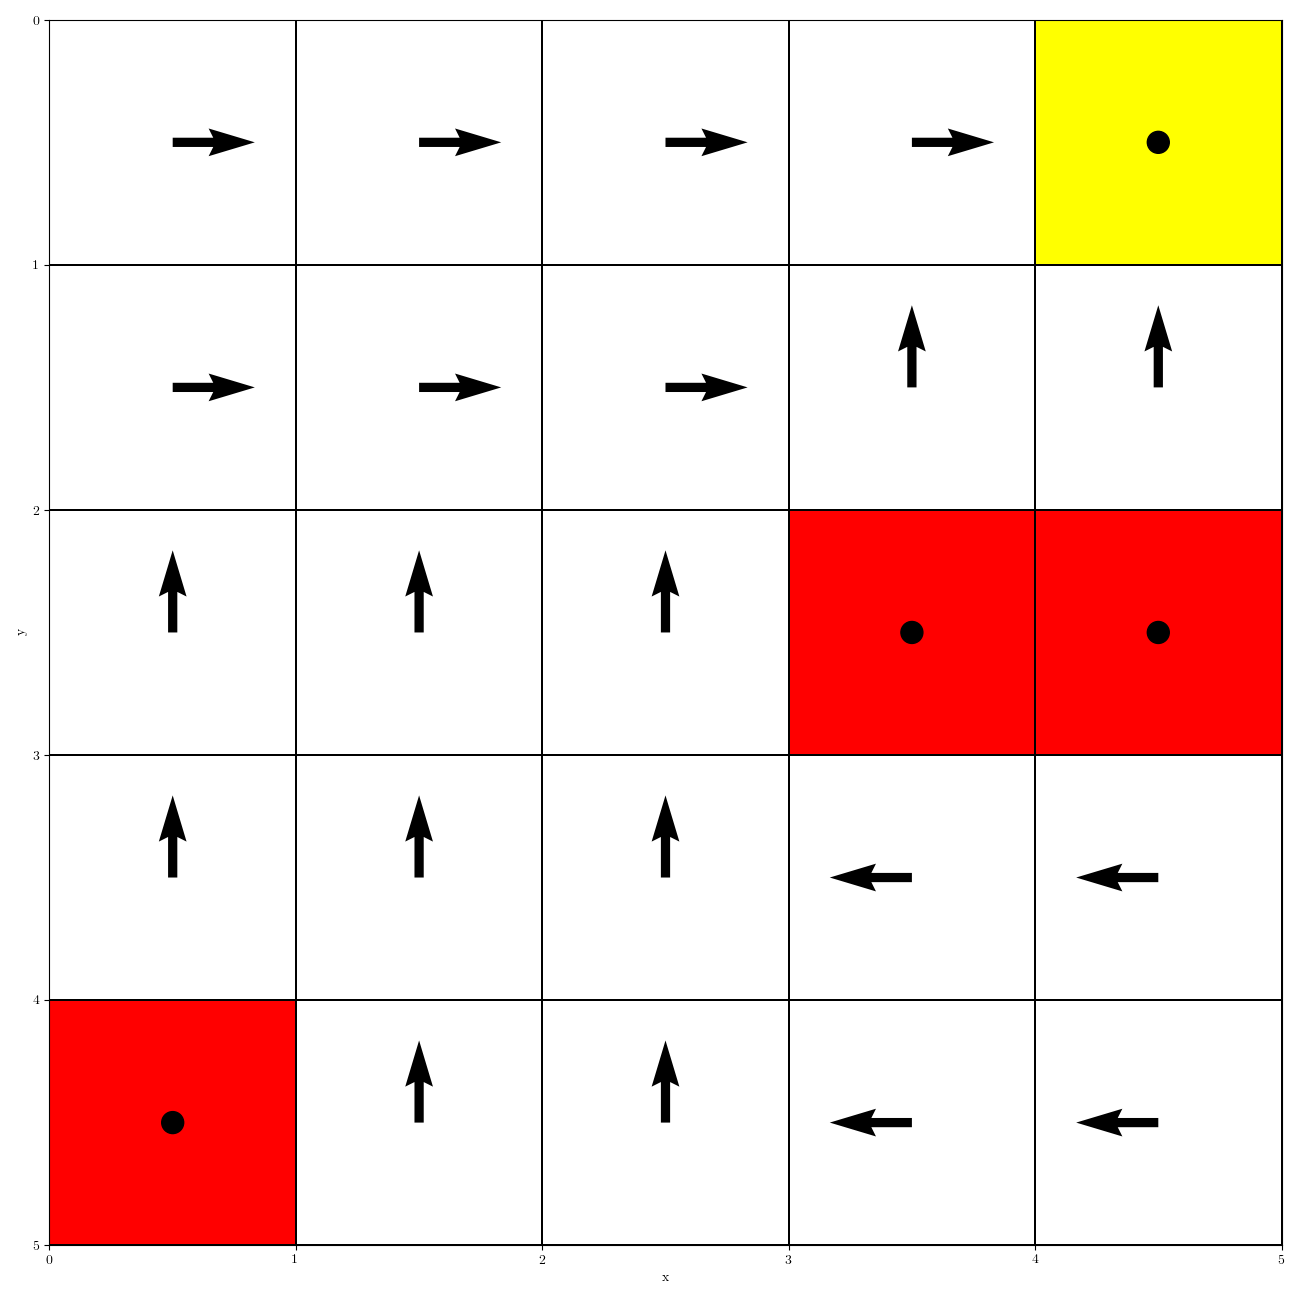
\includegraphics[width=\textwidth]{single_agent_2_policy}
                                \caption{True Policy of \agent{2}.}
                                \label{fig:single_agent_2_policy}
                        \end{minipage}
                }
        \end{center}
    \end{figure}


    \begin{figure}[htb]
        \begin{center}
                \fbox{
                        \begin{minipage}{0.5\textwidth}
                                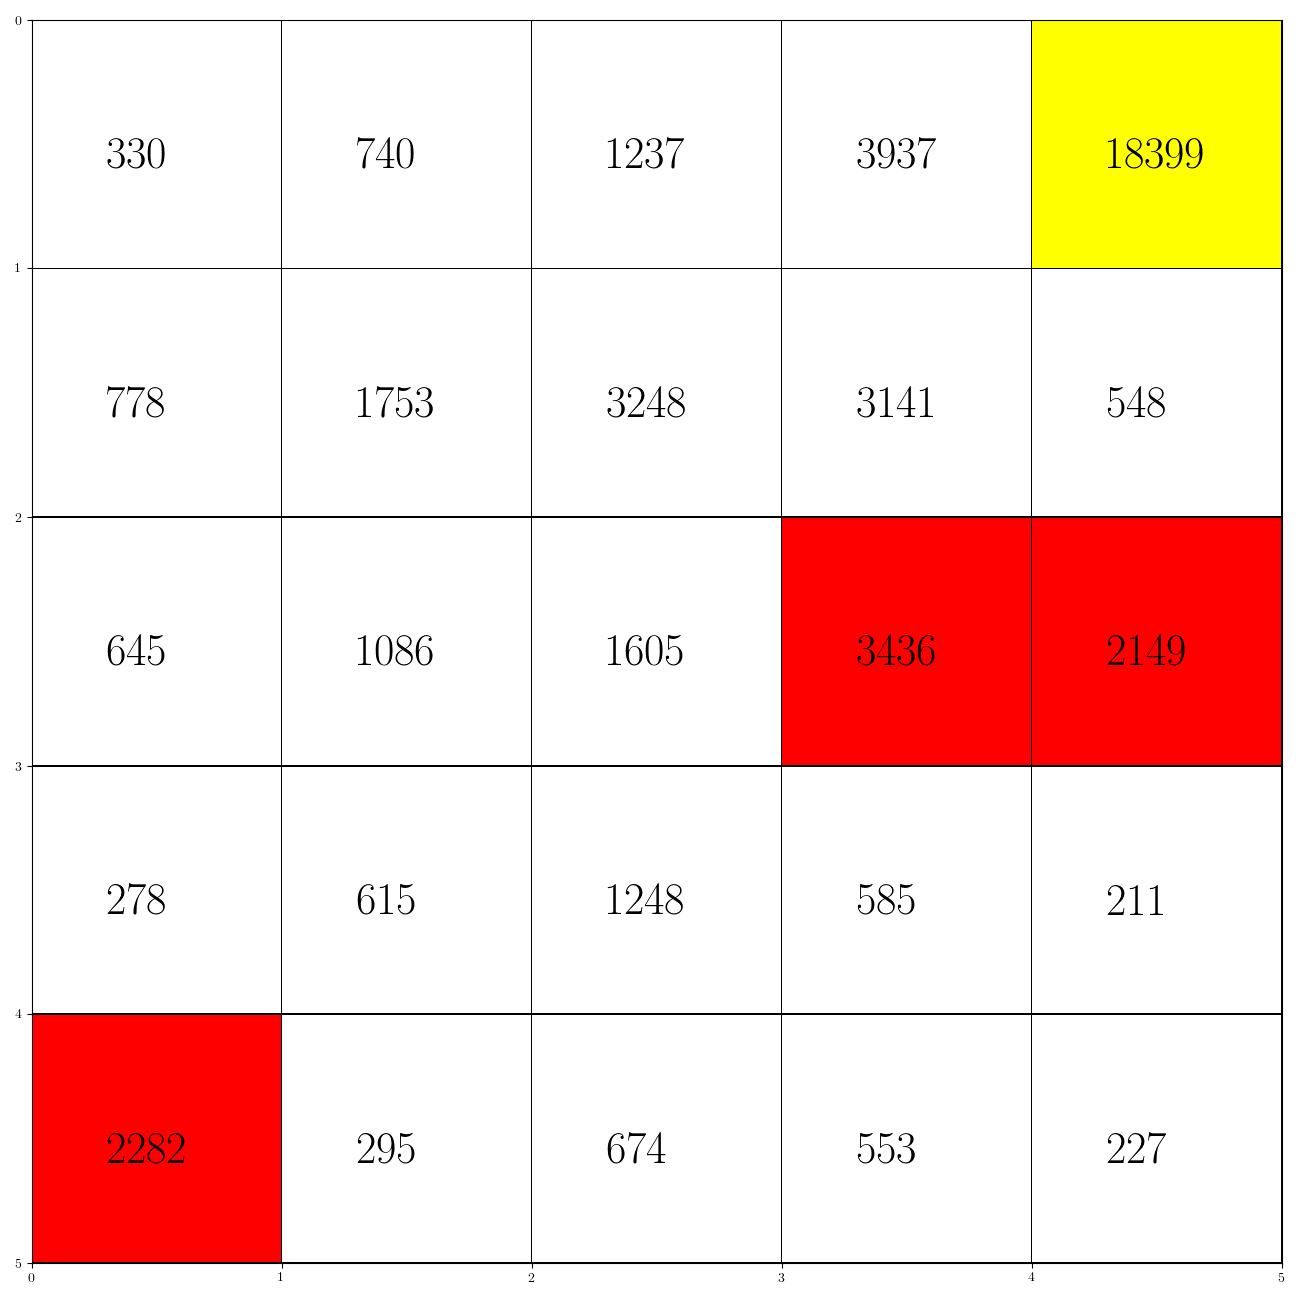
\includegraphics[width=\textwidth]{single_agent_demo}
                                \caption{State visitation count in single agent demonstration.}
                                \label{fig:single_agent_demo}
                        \end{minipage}
                }

        \end{center}
    \end{figure}

    \subsection{Experiment Hyper-parameters}
    To approximate the $Q$-function of \agent{2}, per Section \ref{sec:policy_parameterization}, let's start by placing
    a kernel centered at every grid cell. This sets $W=|S|\times A$, which is an unrealistic number of parameters but
    it's a good test. See Fig.  \ref{fig:kernel_visualization} for a visualization of how the the kernel function
    values, $k(s,a_2)$, at each state are mapped to the feature vector-function $\featFunc$. We'll set the following
    parameters:

    \begin{table}[H]
        \centering
        \begin{tabular}{c|l l}
                $\kernStdDev_{\kernIdx}$ & $1.1,\ \forall l$ & Identical kernel standard-deviations\\
                $\kappa$ & $0.1$ & Temperature of $\estimate{\policy{}}_2$. Eq. (\ref{eq:policy_model}) \\
                $\lambda$ & $1\mathrm{e}\!-\!5$ & Gradient update rate. Eq. (\ref{eq:gradient_update}) \\
                $\eta$ & $0.0$ & Gradient velocity memory\\
                $m$ & 5000 & Per iteration sample size of $\paramVec\sim \rho$\\
                $\Lambda$ & $60$ & Moving average buffer length for $\mathsf{HIST}(\logLike)$ \\
                $\zeta$ & $0.001$ & Gradient ascent termination when $\Delta\mathsf{HIST}(\logLike) < \zeta$\\
                    $\mu_{0}$ & $0.0$ & Initial parameter means\\
                $\nu_{0}$ & $1.0$ & Initial parameter standard-deviations\\
                $\nu_{min}$ & $0.2$ & Minimum parameter standard-deviation\\
        \end{tabular}
        \caption{Hyper-parameters used for single agent inference.}
        \label{table:single_agent_hyper_params}
    \end{table}

    \begin{table}[H]
        \centering
        \begin{tabular}{c|l l}
                $|\traj|$ & $10$ & Number of steps in a trajectory \\
                $|D|$ & $5000$ & Number of trajectories observed \\
                $I_0$ & $\mathcal{U}(0,24)$ & Uniform distribution of $s_2^{(0)}$ \\
        \end{tabular}
        \caption{Observed data for single agent inference.}
        \label{table:single_agent_data_set}
\end{table}

    \begin{figure}[h]
        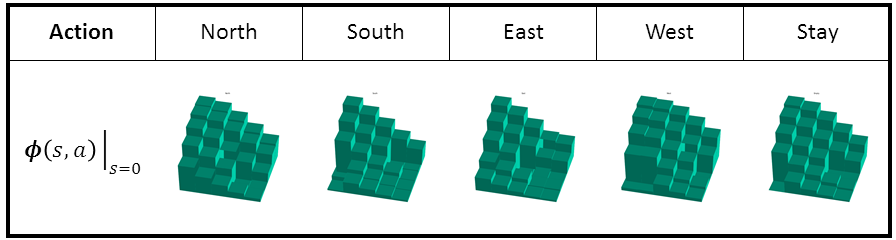
\includegraphics[width=\textwidth]{feature_clarification}
        \caption{Feature values for a kernel centered at cell $0$.}
        \label{fig:kernel_visualization}
    \end{figure}

\subsubsection{Algorithm bounds}

    As noted in footnote 2 of \cite{williams1992simple}, there is not gradient stepsize, $\lambda$ (this reports
    notation), that will keep the parameter variance elements $\nu_w >0$. Our remedy is to enforce a lower bound on the
    covariance of $\rho_n$ after each gradient update in Eq. \ref{eq:gradient_update}:
    \begin{equation}\label{eq:param_var_bounds}
    \nu_{min} \leq \vect{\nu}_n,\ \forall \nu_w \in \vect{\nu}_n.
    \end{equation}

\subsection{Results}\label{sec:single_agent_25K_results}
    Our Assumption \ref{assump:opt_policy_err} is verified by Figures \ref{fig:single_agent_logLike_25_kernels} and
    \ref{fig:single_agent_L1Norm_25_kernels}. The recorded $\mathsf{L}_{\infty}$-norm was neither used during gradient
    ascent, nor as a termination criteria. Note that the final $\mathsf{L}_\infty\text{-norm} \approx 0.7$. This final
    error has a range of about $[0.01-5]$ with these parameters over different trials.  We can also examine the dynamics
    of the distribution $\rho$ as well, see Figures \ref{fig:smooth_gradient_dynamics_mu} and
    \ref{fig:smooth_gradient_dynamics_nu}.

    Note that the legend entry ``$\max_{i \in m}\tilde{\mathcal{L}}_n(D|\mathbf{\theta}^{(i)})$" represents the
    \emph{sampled} parameter vector that maximizes the log-likelihood of $D$ at the iteration $n$. The policy estimate
    $\estimate{\pi}_2(\estimate{\paramVec})$ is constructed using $\mu_N$, the mean vect of the multi-variate
    distribution $\rho$ at the final iteration, $N$.

    As the iterations progress, notice that the parameter variances decrease in Fig. \ref{fig:single_agent_7K_nu},
    implying that the value of of each parameter is known with more confidence.

    \begin{figure}[H]
        \begin{center}
            \fbox{
                \begin{minipage}{0.75\textwidth}
                    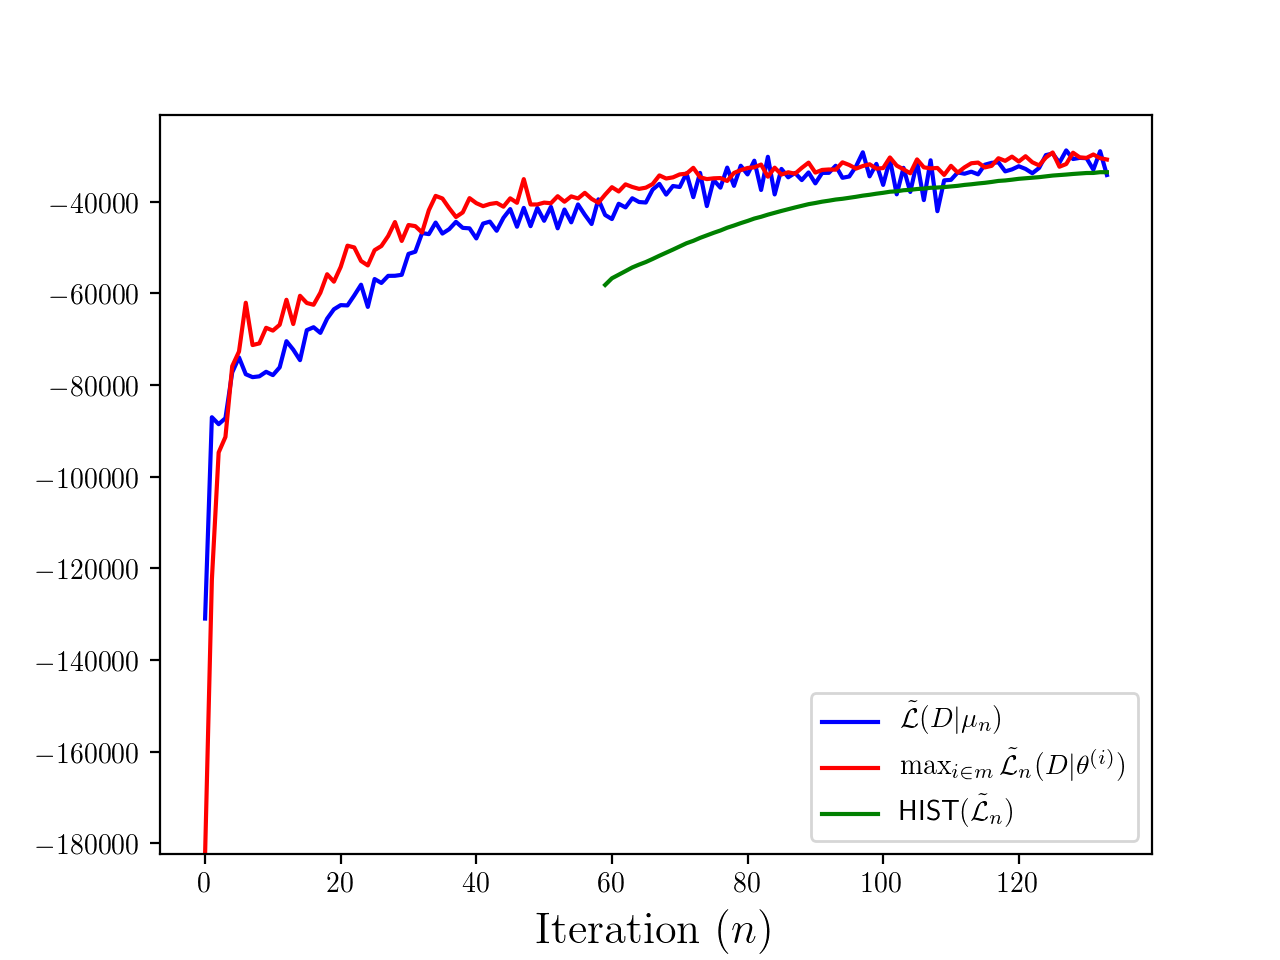
\includegraphics[width=\textwidth]{logLike_25K_temp_0_1}
                    \caption{$\tilde{\logLike}(D|\rho)$ with parameters in Table \ref{table:single_agent_hyper_params}.}
                    \label{fig:single_agent_logLike_25_kernels}
                \end{minipage}
            }
        \end{center}
    \end{figure}

    \begin{figure}[H]
        \begin{center}
                \fbox{
                        \begin{minipage}{0.75\textwidth}
                                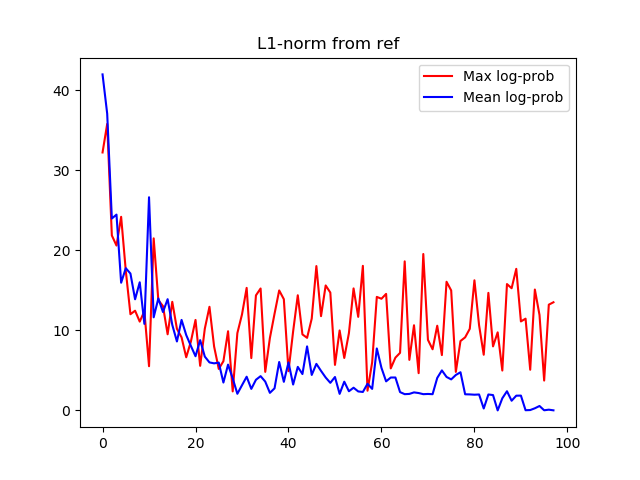
\includegraphics[width=\textwidth]{L1Norm_25K_temp_0_1}
                                \caption{$\OneNorm{\policy{2},\estimate{\policy{}}_2}$ with parameters in Table
                                        \ref{table:single_agent_hyper_params}.}
                                \label{fig:single_agent_L1Norm_25_kernels}
                        \end{minipage}
                }
        \end{center}
    \end{figure}


        \begin{figure}[H]
                \begin{center}
                        \fbox{
                                \begin{minipage}{0.75\textwidth}
                                        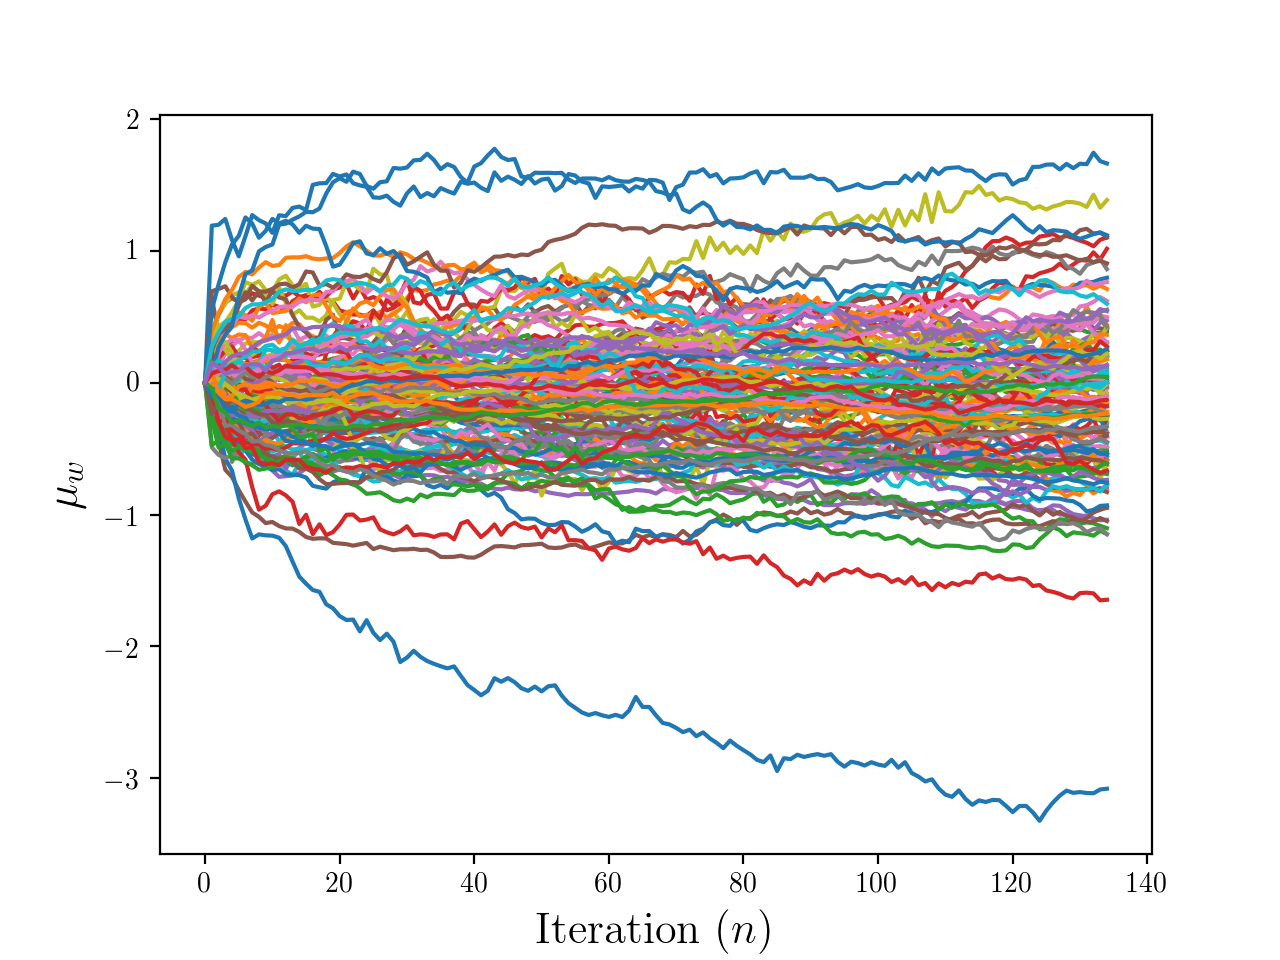
\includegraphics[width=\textwidth]{smooth_grad_descent_mu}
                                        \caption{$\mu_w$ for each iteration with parameters in Table
                                                \ref{table:single_agent_hyper_params}.}
                                        \label{fig:smooth_gradient_dynamics_mu}
                                \end{minipage}
                        }
                \end{center}
        \end{figure}

        \begin{figure}[H]
        \begin{center}
                \fbox{
                        \begin{minipage}{0.75\textwidth}
                                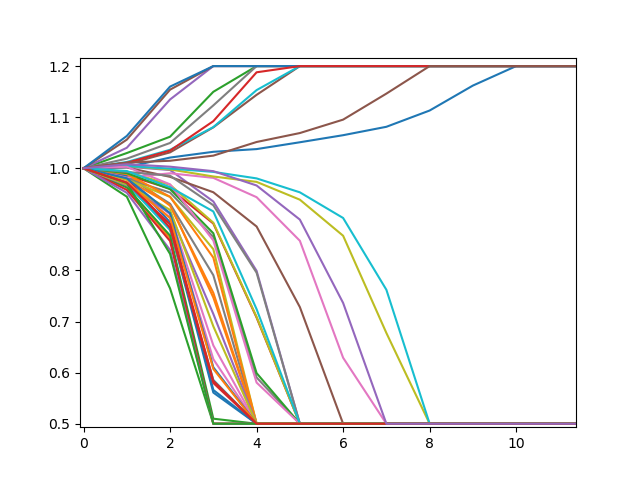
\includegraphics[width=\textwidth]{smooth_grad_descent_nu}
                                \caption{$\nu_w$ for each iteration with parameters in Table
                                        \ref{table:single_agent_hyper_params}.}
                                \label{fig:smooth_gradient_dynamics_nu}
                        \end{minipage}
                }
        \end{center}
        \end{figure}

    \subsection{Experiment with Fewer Kernels}

        Note that if we use $K=7$, and use the parameters in Table \ref{table:single_agent_new_hyper_params}, we can
        achieve a final $\mathsf{L}_{\infty}\text{-norm} \approx 6.5$. There is some obvious generalization error in the
        inferred policy shown in Fig. \ref{fig:single_agent_policy_7_kernels}. Note that the grid-cells with blue
        circles in them note only that a kernel is centered at that location, the circle is not proportional to
        $\kernStdDev_{\kernIdx}$. Also, the magnitudes of the circles and arrows are proportional to the probability of
        selecting that action; the yellow cell is in the most North-East cell.

\todo[inline]{Format this table similar to Table \ref{table:single_agent_hyper_params}.}
    \begin{table}[H]
        \centering
        \begin{tabular}{c|c}
                $\kernStdDev_{\kernIdx}$ & $\mathbf{2.0},\ \forall l$ -- Identical kernel standard-deviations.\\
                $\kappa$ & $0.1$ -- Temperature of $\estimate{\policy{}}_2$. Eq. (\ref{eq:policy_model}). \\
                $\lambda$ & $\mathbf{1\mathrm{e}\!-\!6}$ -- Gradient update rate. Eq. (\ref{eq:gradient_update}) \\
                $\eta$ & $\mathbf{0.2}$ -- Gradient velocity memory.\\
                $m$ & 5000 -- Per iteration sample size of $\paramVec\sim \rho$.\\
                $\Lambda$ & $60$ - Moving average buffer length for $\mathsf{HIST}(\logLike)$. \\
                $\zeta$ & $0.001$ Gradient ascent termination when $\Delta\mathsf{HIST}(\logLike) < \zeta$.\\
                $\nu_{min}$ & $0.2$ -- Minimum parameter standard-deviation.\\
        \end{tabular}
        \caption{Hyper-parameters for inference with $K=7$.}
        \label{table:single_agent_new_hyper_params}
    \end{table}

    \begin{figure}[htb]
        \begin{center}
            \fbox{
                \begin{minipage}{0.75\textwidth}
                    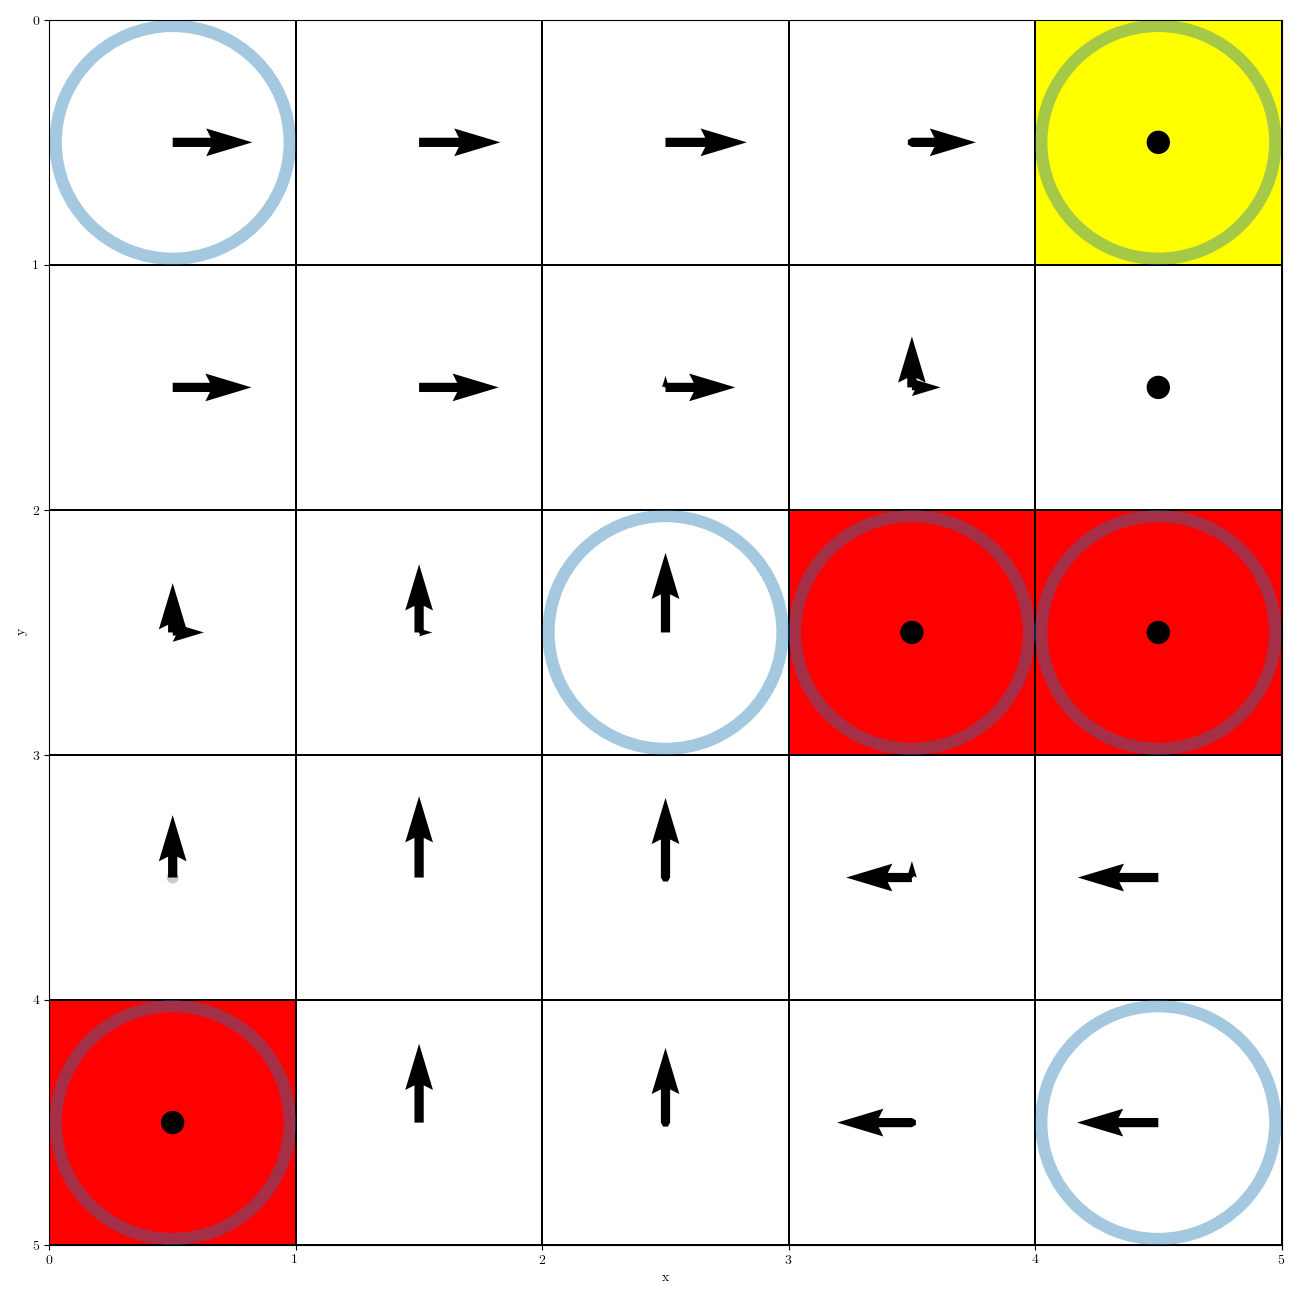
\includegraphics[width=\textwidth]{single_agent_learned_7Kernels}
                    \caption{$\estimate{\policy{}}_{2}$ with parameters in Table
                             \ref{table:single_agent_new_hyper_params}.}
                    \label{fig:single_agent_policy_7_kernels}
                \end{minipage}
            }
        \end{center}
    \end{figure}

    \begin{figure}[htb]
        \begin{center}
            \fbox{
                \begin{minipage}{0.75\textwidth}
                    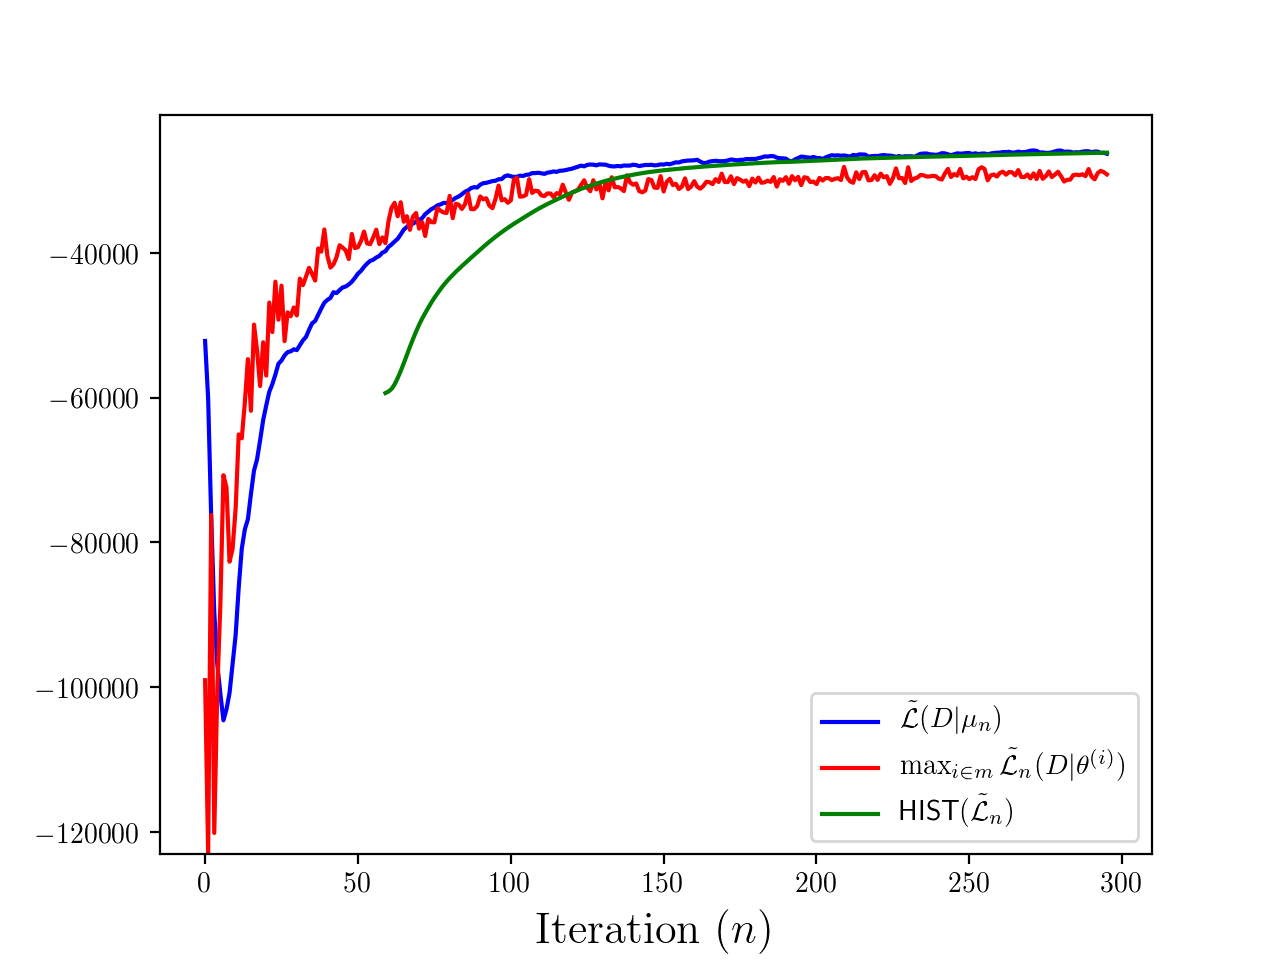
\includegraphics[width=\textwidth]{Loglike_single_agent_7K}
                    \caption{$\tilde{\logLike}(D|\rho)$ with parameters in Table
                             \ref{table:single_agent_new_hyper_params}.}
                    \label{fig:single_agent_logLike_7_kernels}
                \end{minipage}
            }
        \end{center}
    \end{figure}


    \begin{figure}[H]
        \begin{center}
                \fbox{
                        \begin{minipage}{0.75\textwidth}
                                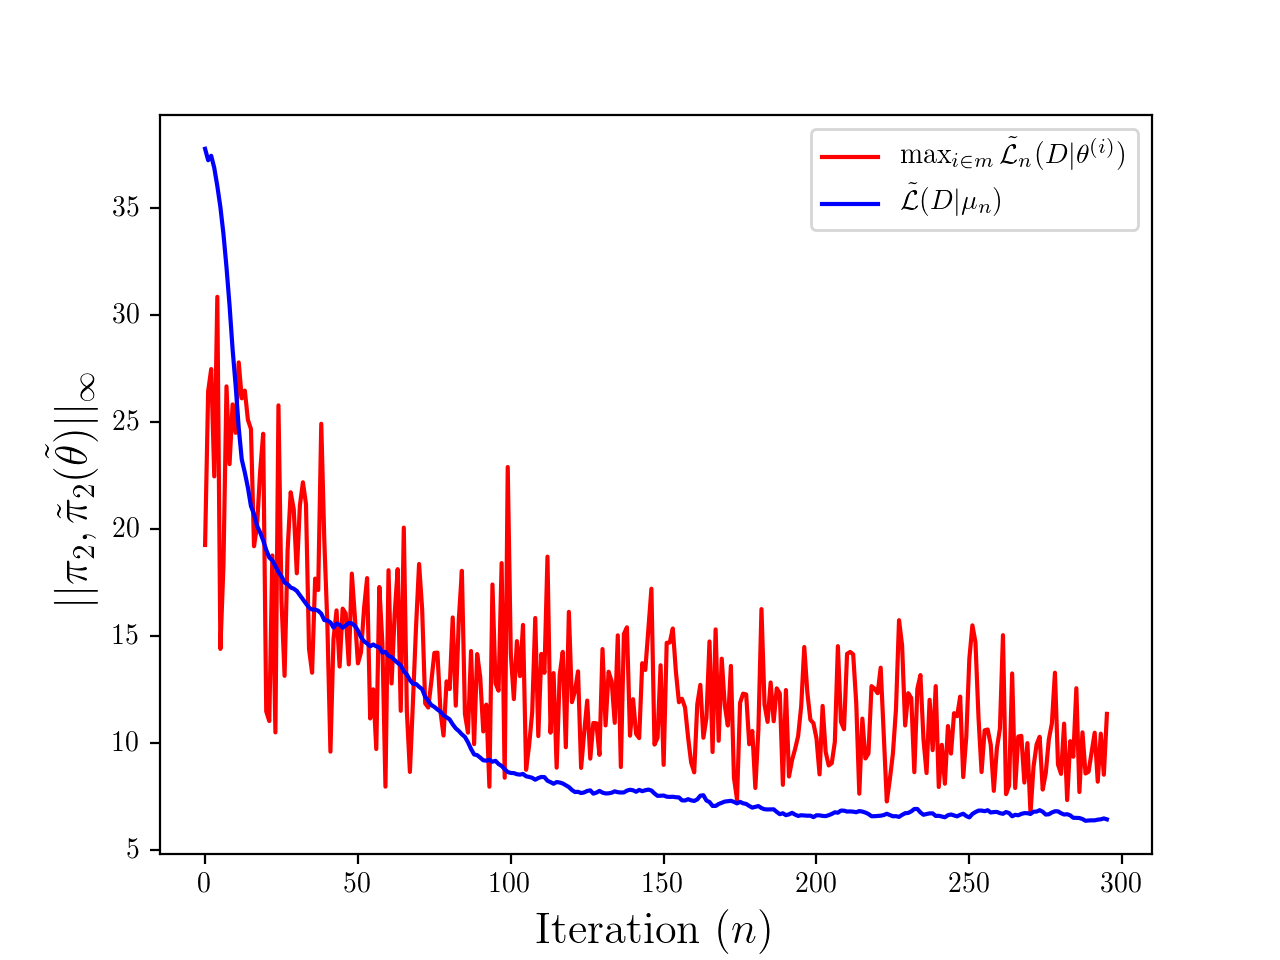
\includegraphics[width=\textwidth]{Linf_norm_single_agent_7K}
                                \caption{$\OneNorm{\policy{2},\estimate{\policy{2}}}$ with parameters in Table
                                        \ref{table:single_agent_new_hyper_params}.}
                                \label{fig:single_agent_L1Norm_7_kernels}
                        \end{minipage}
                }
        \end{center}
\end{figure}

    \begin{figure}[htb]
        \begin{center}
                \fbox{
                        \begin{minipage}{0.75\textwidth}
                                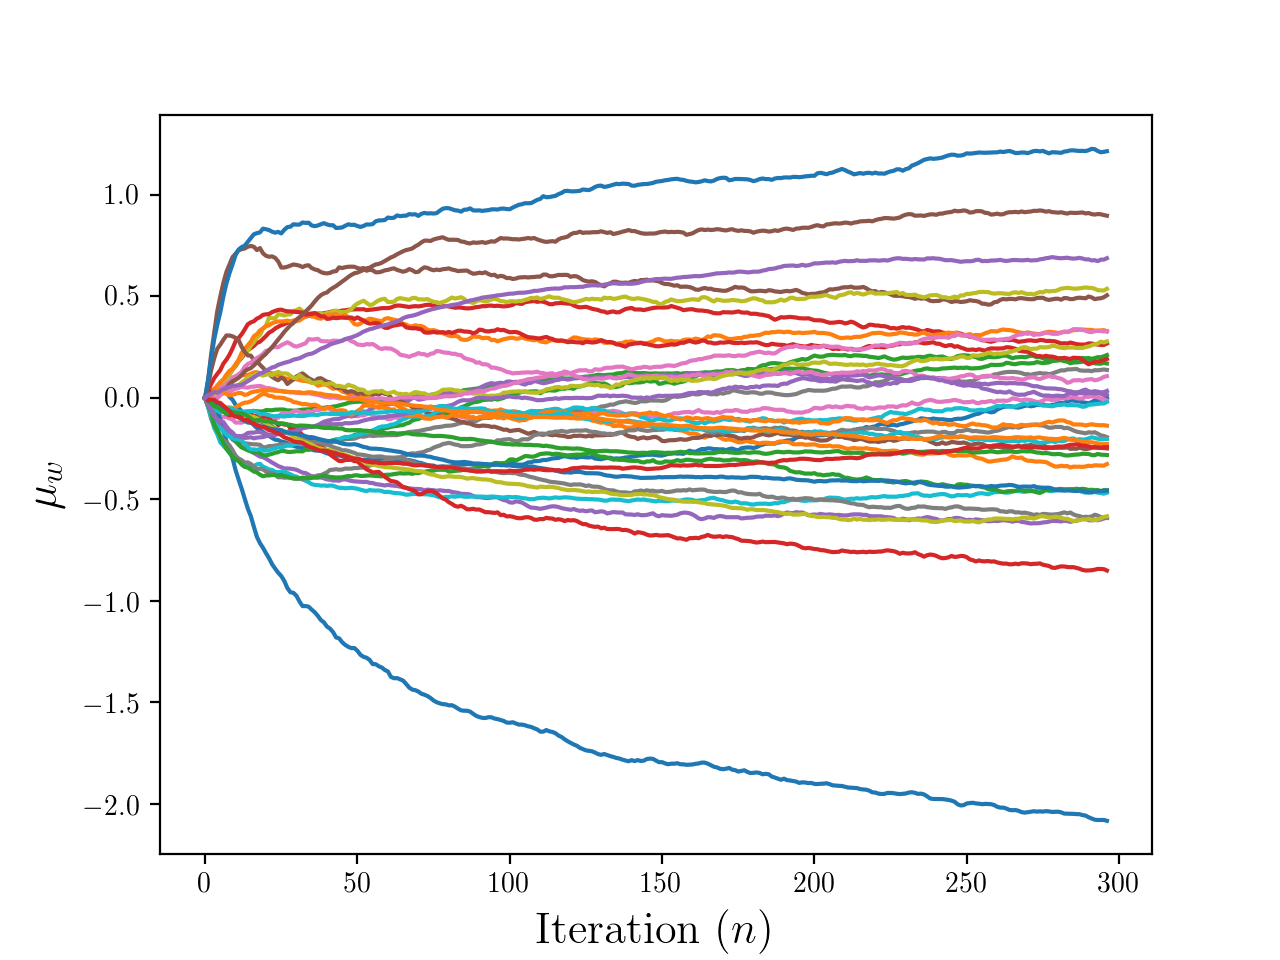
\includegraphics[width=\textwidth]{grad_descent_mu_7K}
                                \caption{$\mu_w$ with parameters in Table
                                        \ref{table:single_agent_new_hyper_params}.}
                                \label{fig:single_agent_7K_mu}
                        \end{minipage}
                }
        \end{center}
    \end{figure}


    \begin{figure}[htb]
        \begin{center}
                \fbox{
                        \begin{minipage}{0.75\textwidth}
                                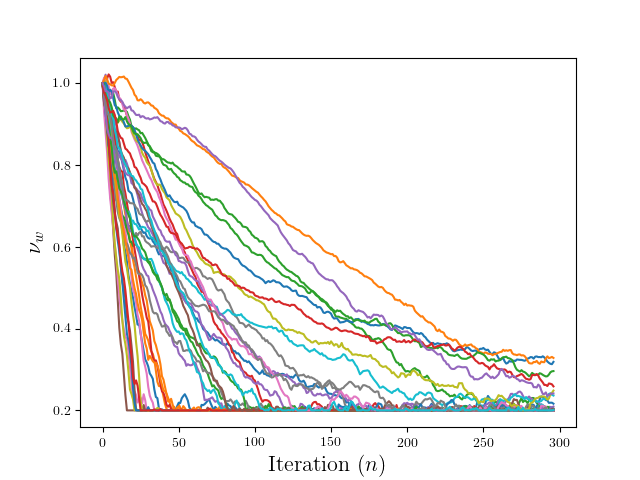
\includegraphics[width=\textwidth]{grad_descent_nu_7K}
                                \caption{$\nu_w$ with parameters in Table
                                        \ref{table:single_agent_new_hyper_params}.}
                                \label{fig:single_agent_7K_nu}
                        \end{minipage}
                }
        \end{center}
\end{figure}





\chapter{Expectation Maximization for Policy Iteration}\label{chapt:policy_iteration}
        This is mostly a presentation of results from an implementation of \cite{toussaint2010expectation}.

        If the hidden parameter, $\pi_2$ was known, then the discout optimal policy to fulfill the robots task,
        \optimal{\pi_1} could be completely solved \cite{hernandez2012adaptive}:

\chapter{Proactive Policy Inference}\label{chapt:proactive_inference}

    Assuming that \agent{1} has received some initial data $D^{(1)}$, the estimated policy of the uncontrollable agent
    can be improved from some initial guess $\estimate{\policy{}}_2^{(0)}$ to form $\estimate{\policy{}}_2^{(1)}$. Let's
    assume that $D^{(1)}$ was incomplete, it did not contain enough data for the following algorithm to meet the
    tolerance required by Assumption \ref{assump:opt_policy_err}. Therefore, \agent{1} will need to gather more data,
    trajectories, $D^{(b)},\ b=1,\ldots,B$. Ideally, $D^{(b)}$ will contain data that were lacking in all previous
    batches. When there are not enough data, some estimates parameter elements, $\estimate{\theta}_\paramIdx$, will be
    incorrect. The parameter vector inferred from any batch will be written $\estimate{\paramVec}^{(b)}$, which is not
    to be confused with the sampled $\paramVec^{(i)}$ in Eq. \ref{eq:gradLogLike}. There are two options for
    incorporating $D^{(1)}$ into the next batch.

    First, the policy update to $\policy{1}^{(1)}$ can include only $\estimate{\policy{}}_2^{(1)}$; \agent{1} will
    simply exploit the information from $D^{(1)}$ so that $\policy{2}^{(1)}$ maximizes the expected discounted reward,
    as shown in Section \ref{sec:ADO_policy}. Since the transition function $T(s'|s,(a_1,a_2)) $ is stochastic, some new
    data will probably be observed. This is considered to be a \textit{passive} algorithm, shown in Algorithm
    \ref{alg:passive_mini_batch}.
    \todo[inline]{improve algorithm description}
    \begin{algorithm}\label{alg:passive_mini_batch}
        set $\estimate{\policy{}}_2^{(0)}(s,a_2) = \mathcal{U}$;\\
        \For{$b \in [1,B]$}{
            Solves for $\policy{1}^b(s, \estimate{\policy{}}_2^{(b-1)} )$;\\
            Initialize demonstration set $D=\emptyset$;\\
            \For{$d\ \in |D|$}{
                \For{$t=0\ to\ |\traj_d|$}{
                    The robot plays policy $\policy{1}^b$ and the environment plays the true \policy{2};
                    Record $\traj_t = (s_1, s_2)$;
                }
                Add $\traj_d$ to $D$;
            }
            Infer $\estimate{\policy{}}_2^{(b)}$;
        }
        \caption{Passive-inference in Mini-batches}
    \end{algorithm}

     \par
     The second option is for \agent{1} to \textit{proactively} seek the most informative $D^{(1)}$.  Gathering data
     about any unknown parameter elements will be given to \agent{1} as a bonus reward; \agent{1} proactively improves
     the inference of $\estimate{\policy{}}_2$. Therefore, \agent{1} needs to determine which
     $\estimate{\theta}_\paramIdx$\!'s are unknown.

\section{Characterizing Unknown Parameters}\label{sec:unknown_params}
    In the problem formulation, the transition function is jointly determined by the robot and the environment agent.
    \[
    P((s_1',s_2')|(s_1,s_2),(a_1,a_2)) = T(s_1'|s_1,a_1) \policy{2}(a_2|(s_1,s_2))
    \]
    If $\pi_2(a_2|(s_1,s_2))$ is state-dependent policy \textcolor{blue}{and non approximate solution is sort(sort
    ???)}, then learning the dynamics of the MDP is equivalent to learning the policy $\policy{2}$. And both problems
    have the same sample complexity, they are polynomial in the size of the joint state space and the action space of
    the \agent{2}.  With the Gaussian policy approximation from Section \ref{sec:gauss_policy}, if the number of
    parameters, $W$ is much less than $\abs{|S|\times A}$, then sample complexity will be reduced significantly.

    Since the policy parameter estimate $\estimate{\paramVec}$ is a collection of Gaussian random variables, for each
    state-action pair $s = (s_1,s_2)\in S$ and $a_2\in A$, we have \[
    \estimate{\policy{}}_2(a_2| s) \propto \exp\left[Q(s,a_2;\estimate{\paramVec}) - V(s;\estimate{\paramVec})\right].
    \]
    %https://instream.zendesk.com/hc/en-us/articles/202386009-What-is-the-difference-between-a-Normal-Distribution-and-a-Lognormal-Distribution-
    Since $Q(s,a;\estimate{\paramVec})$ is a Gaussian random variable with certain mean and variance, the exponential
    the \textit{Q}-function is a lognormal random variable.  Therefore, $V(s;\estimate{\paramVec})$ is a summation of
    lognormal random variables $V(s)=\kappa \log \sum\exp (Q(s,a;\estimate{\paramVec})/\kappa)$; it also is known that
    the sum of lognormal random variables can be approximated by a lognormal random variable, denoted $Q^\ast(s,a
    ;\uptheta)$.
    \todo[inline, color=green]{$Q^\ast$ appears to be unused. Is this necessary?}

    \textcolor{blue}{Next: can we generate the mean and variance of the $\pi_2(a|s)$ and use it to determine the bonus reward?}

    \begin{definition}
        Given two parameters $\epsilon, \varphi \in (0,1)$, a parameter $\theta_{\paramIdx}$ is $(\epsilon,
        \varphi)$-known if with probability $1-\varphi$, the probability of the true value for $\paramElem$ is
        $\epsilon$ close to the mean of the Gaussian distribution $\normal{\mu_{\paramIdx}, \nu_{\paramIdx}}$, \ie,
        \[
        P(\abs{\paramElem - \mu_{\paramIdx}} \ge \epsilon) \le \varphi.
        \]
    \end{definition}
    When the estimated unknown policy parameter $\paramElem$ is $\epsilon$-close to the mean $\mu_{\paramIdx}$ with
    probability $1-\varphi$, then we consider enough knowledge has been obtained for $\paramElem$ and treat it as a
    \emph{known} policy parameter.

    Let $\Theta_\known$ be the set of known policy parameters and $\Theta_{\unknown}$ be the remaining unknown
    parameters.  Next, we present a method that enables to determine whether a state is unknown from the knowledge of
    $\Theta$.

    First, given that $\paramVec_i$ is a Gaussian variable, the $Q$ function for a pair of state-action $(s,a)$ is
    \[
    Q(s,a ;\uptheta) \sim \sum_{i=1}^N \phi_i(s,a) \normal{\mu_i, \sigma_i^2}
    \]
    where $\phi_i(s,a),i=1,\ldots, N$ can be viewed as the mixing parameters.
    \todo[inline, color=green]{I would like to rewrite the preceding sentence as I have below. Is my interpretation
    correct? My next green comment is (potentially) also related to this.}

    \emph{First, given that each sampled parameter vector in Eq. \ref{eq:gradLogLike}, $\paramVec^{(i)}$, is a Gaussian
          variable, the $\estimate{Q}$-function is
          \[
          \estimate{Q}(s,a ;\paramVec^{(i)}) \sim \sum_{w=1}^W \featElem(s,a_2) \normal{\mu_w, \nu_w^2}
          \]
          where $\featElem(s,a_2),\ w=1,\ldots, W$ can be viewed as the mixing parameters. }

    A state $s$ is known if and only if for any $a_2 \in A$, $Q(s,a_2)$ is known. Since the $Q$-value is a mixture of
    Gaussians, the mean and variance of $Q(s,a;\estimate{\paramVec}^{(b)})$ can be computed and used after each batch of
    new data to determine the distribution of a random variable -- the estimate of $\policy{2}(a|s)$.

    If we were trying to solve a Probably-Approximatly-Correct- (PAC)-MDP, we would require a desired accuracy in
    learning the transition function, for example, $\bar T(s'|s,a_1) - T(s'|s,a_1) \le \varepsilon$ with probability
    $1-\varphi$, where $\bar T$ is the estimated transition function and $T$ is the true transition function.

    Based on the needed accuracy and the relation between $T$ and $\policy{2}$,
    \[
    P(s'|s,a_1) = T(s'|s,(a_1,a_2))\pi_2(a_2|s),
    \]
    we can show:
    \begin{align*}
        \bar P(s'|s,a_1)  -P(s'|s,a_1)
        & = T(s'|s,(a_1,a_2))\left( \pi_2(a_2|s) - \bar \pi_2(a_2|s)
        \right)\\
        & \approx T(s'|s,(a_1,a_2))\big(\exp(Q(s,a_2)-V(s)) - \exp(Q(s,a_2;\paramVec^{(b)})-V(s;\paramVec^{(b)})) \big)
    \end{align*}

    Since $Q(s,a_2;\paramVec)$ is a Gaussian, $\exp Q(s,a_2;\paramVec)$ is log-normal, ${V =\log \exp \sum
    Q(s,a;\paramVec)}$ can be approximated as a Gaussian (similar to approximating hardmax with softmax, but here we
    approximate $V$ by $\max_a Q(s,a)$). Given this knowledge, we can quantify the bounded error between the estimated
    transition and true transition by analyzing the distribution of random variable
    $\exp(Q(s,a_2;\uptheta)-V(s;\theta))$.

    \todo[inline, color=green]{Is there a significance to using 'uptheta' in the Q-function vs 'theta' in the Value
    function above? I've replaced several of them with 'paramVec' since I was thinking we only needed to differentiate
between $\paramVec$ and $\Theta$ ('Theta')...}

    \todo[inline,color=green]{
        Is this section more justification for our method for building the bonus reward or does it show that we only
        need to sample the "policy-space" since we've shown \policy{2} is a Gaus-RV? In that case, what do we consider
        samples? Is $\policy{2}(s;\paramVec^{(i)})$ (Eq \ref{eq:gradLogLike}) a sample, or is
        $\policy{2}^{(b)}(s,\estimate{\paramVec}^{(b)})$ a sample (Alg. \ref{alg:passive_mini_batch})?
        }

    \color{blue}
    While I was trying to figure out what we consider ``samples", I thought of a related way to determine if \paramElem
    should be in $\Theta_\known$. If we record all (or a subset of) the $n=1,\ldots,N$ values of $\rho^n = (\mu_n,
    \nu_n)$ from in each iteration of the gradient ascent algorithm (see Eq. \ref{eq:gradient_update} and the first
    sentence of Sec. \ref{sec:policy_infer_terminate}) we can analyze Shannon's Entropy of the samples generated in the
    $b$-th inference of \policy{2} relative to the distribution of the final iteration ($N$):
    \[
    \mathcal{H}(\paramElem^{(b)}) = - \sum_{n=1}^{N} p(\mu_n| \rho_N)\log p(\mu_n|\rho_N).
    \]
    If a parameter is \emph{known} from a previous batch $b-1$, then we expect this $\paramElem^{(b)}$ not to change
    very much, therefore it will have a very low entropy. If it is unknown, then the mean value $\mu_w$ will slowly
    wander around a lot and have a very high entropy see Fig. \ref{fig:bad_gradient_dynamics_nu} vs (Fig.
    \ref{fig:smooth_gradient_dynamics_nu}.  and Fig. \ref{fig:fast_gradient_dynamics_nu}).

    \par
    This idea is definitely motivated by my use of Eq. \ref{eq:param_var_bounds} due to the numerical stability issues.
    \color{black}


\subsection{Bonus Reward}

    \todo[inline,color=green]{See changes from $\delta R(s,a_2)$ to $\delta R(s)$ here}
    Per Eq. \ref{eq:QFuncApprox} the policy $Q(s,a) = \sum_{w=1}^{\paramLen} \theta_w \phi(s,a)$ so $\pi(s,a)\propto
    \exp(Q(s,a)/\traj)$. Given the Gaussian distributions of $\paramVec$ from Sec. \ref{sec:unknown_params}, the Q-value
    has a variance
    \[
    \Omega(s,a_2)=\sum_{w=1}^{\paramLen} \nu_w^2 \phi_w^2(s,a_2).
    \]
    What we would like to do is give \agent{1} a bonus reward whenever \agent{2} takes an action for which
    $\estimate{Q}(s,a_2)$ has a large $\Omega(s,a_2)$. Since \agent{1} can not actually controll \agent{2} to take an
    ``uncertain" action $a_2$ at a joint state $s$, we build an exploration bonus reward at each joint state.

    Using the original reward function of the robot from Def. \ref{def:hipmdp}, the reward including an exploration
    bonus is defined as
    \[
    \hat R (s,a) = R(s,a) + \delta R(s)
    \]
    and
    \[\delta R(s)  \propto \sum_{a_2\in A}\sum_{\theta_w\in \Theta_\unknown} \nu_w^2 \phi^2_w(s,a_2)
    \]
    In practice, we can select a constant $B$ and define
    \[
    \delta R(s) = B \sum_{a_2\in A}\sum_{\theta_w\in \Theta_\unknown} \nu_w^2 \phi_w^2(s,a).
    \]
    The constant $B$ has a role of weighting between exploration and exploitation.

    \par
    The exploration bonus has the following property: When all parameters becomes known, the exploration bonus will
    become zero and the policy recovers to the optimal policy with respect to the original reward function. By
    definition, for the same estimate of  $\paramVec$, and for any two pairs $(x,a_1), (y,a_2),\ \forall\ x,y\in S_2 | x
    \neq y$, the uncertainty in $Q(x,a_1)$ is greater than that of $Q(y,a_2)$ if $\sum_{a_2\in A}\sum_{\theta_w\in
    \Theta_\unknown} \nu_2^2 \phi^2_w(x,a_2) > \sum_{a_2\in A}\sum_{\theta_w\in \Theta_\unknown}  \nu_w^2
    \phi^2_w(y,a_2)  $, and thus exploring any joint states $s=(s_1,x), \forall s_1 \in S_1$ will receive a higher
    exploration bonus.


\section{Multi-agent Policy Model}

    For the example tasks described in Chapter \ref{chapt:motivation}, a human would infer that the uncontrollable
    agents would only change their actions if the controllable agent is within a relative distance. Other cars might
    only swerve away from a driver if two cars become dangerously close. Alternatively, a human holding a basket might
    only extend their arms to accept a load of items when the manipulator is sufficiently close to them.

\subsection{Fixed and Mobile kernels for policy inference}\label{sec:fixed_and_mobile_kernels}

    \begin{assumption}\label{assump:multi_agent_interraction}
        The uncontrollable agent, \agent{2}, has a nominal policy, and when the agents are within some unknown distance
        $\mathsf{x}$, \policy{2} is biased either towards or away from the position of \agent{1}:
        \begin{align*}
            \policy{2} & = \begin{cases}
                               f(s_2) & \text{if}\ \textnormal{SP}(s_1,s_2) > \mathsf{x} \\
                               f(s_1,s_2) & \text{if}\ \textnormal{SP}(s_1,s_2) \leq \mathsf{x}.
                           \end{cases} \\
        \end{align*}
    \end{assumption}

    Using Assumption \ref{assump:multi_agent_interraction}, then we can segment our parameter and feature vectors into
    fixed and mobile elements. The fixed kernels are still scattered at locations $c_l \subset S_2,\ l=0,\ldots,K-1$.
    Now, consider a mobile kernel that is attached to the \agent{1}\!'s location. When this kernel is far from the
    current state of \agent{2} its anticipated influence is very small due to Eq. \ref{eq:kernel_func}. This simply
    requires that another $|A|$ parameters elements are included in \paramVec.


\chapter{Conclusion}\label{chapt:conclusion}

This thesis has successfully designed a new parameter-based policy inference algorithm that can be used in model-based
\ac{RL}. We applied policy-gradient techniques to maximize the likelihood of observed state-sequences from an
uncontrollable agent with an unknown policy, given a parametric estimate of that policy.

By assuming that the parameter vector is distributed as a multi-variate normal distribution, the policy inference
algorithm captures the parameter variance, which we show can quantify the uncertainty in the estimated \emph{Q}-function
of the uncontrollable agent. This report approximated the \emph{Q}-function as a linear combination of parameters and
features and we successfully demonstrated that we can infer an agent's policy using a feature space that is much smaller
in cardinality than the state-action space.


Using the parametric uncertainty, we also provided two platforms for interacting with an uncontrollable agent. First, if
we're allowed to ask for policy demonstrations, trajectories, from the uncontrollable agent and select the initial state
of the trajectory, we can actively seek to aggregate more informative data and improve the sample efficiency of the
inference. We  can the initial state of a new trajectory based on the estimated variance of the \emph{Q}-function. This
was applied to a single-agent scenario where we learned the agent's policy from demonstration. We discussed that this
active-re-sampling can be used to provide more insight into features that have a high parameter uncertainty. The
single-agent active inference algorithm can accelerate the policy inference, but is highly dependent on the feature
selection.

Second, in a multi-agent experiment, we defined a new bonus-reward that is a function of the estimated variance of the
uncontrollable agent's \emph{Q}-function. This bonus reward convinced a controllable agent to choose actions that led to
informative interactions and accelerated the policy inference of the uncontrollable agent. We discussed future work that
will lead to the controllable agent eventually exploiting the improved information so that it can plan an optimal policy
as soon as possible.



% Now come appendices, if you had any.
% Appendices are automatically numbered, just like everything else in
% LaTeX. But only after you gave this command
\appendix
\chapter{}
\section{8-by-8 Grid World}
This figure shows an example initial data set, $D^{(0)}$ used in line $3$ of Algorithm \ref{alg:single_agent_single_update}.


\begin{figure}[htb]
	\begin{center}
		\fbox{
			\begin{minipage}{0.7\textwidth}
				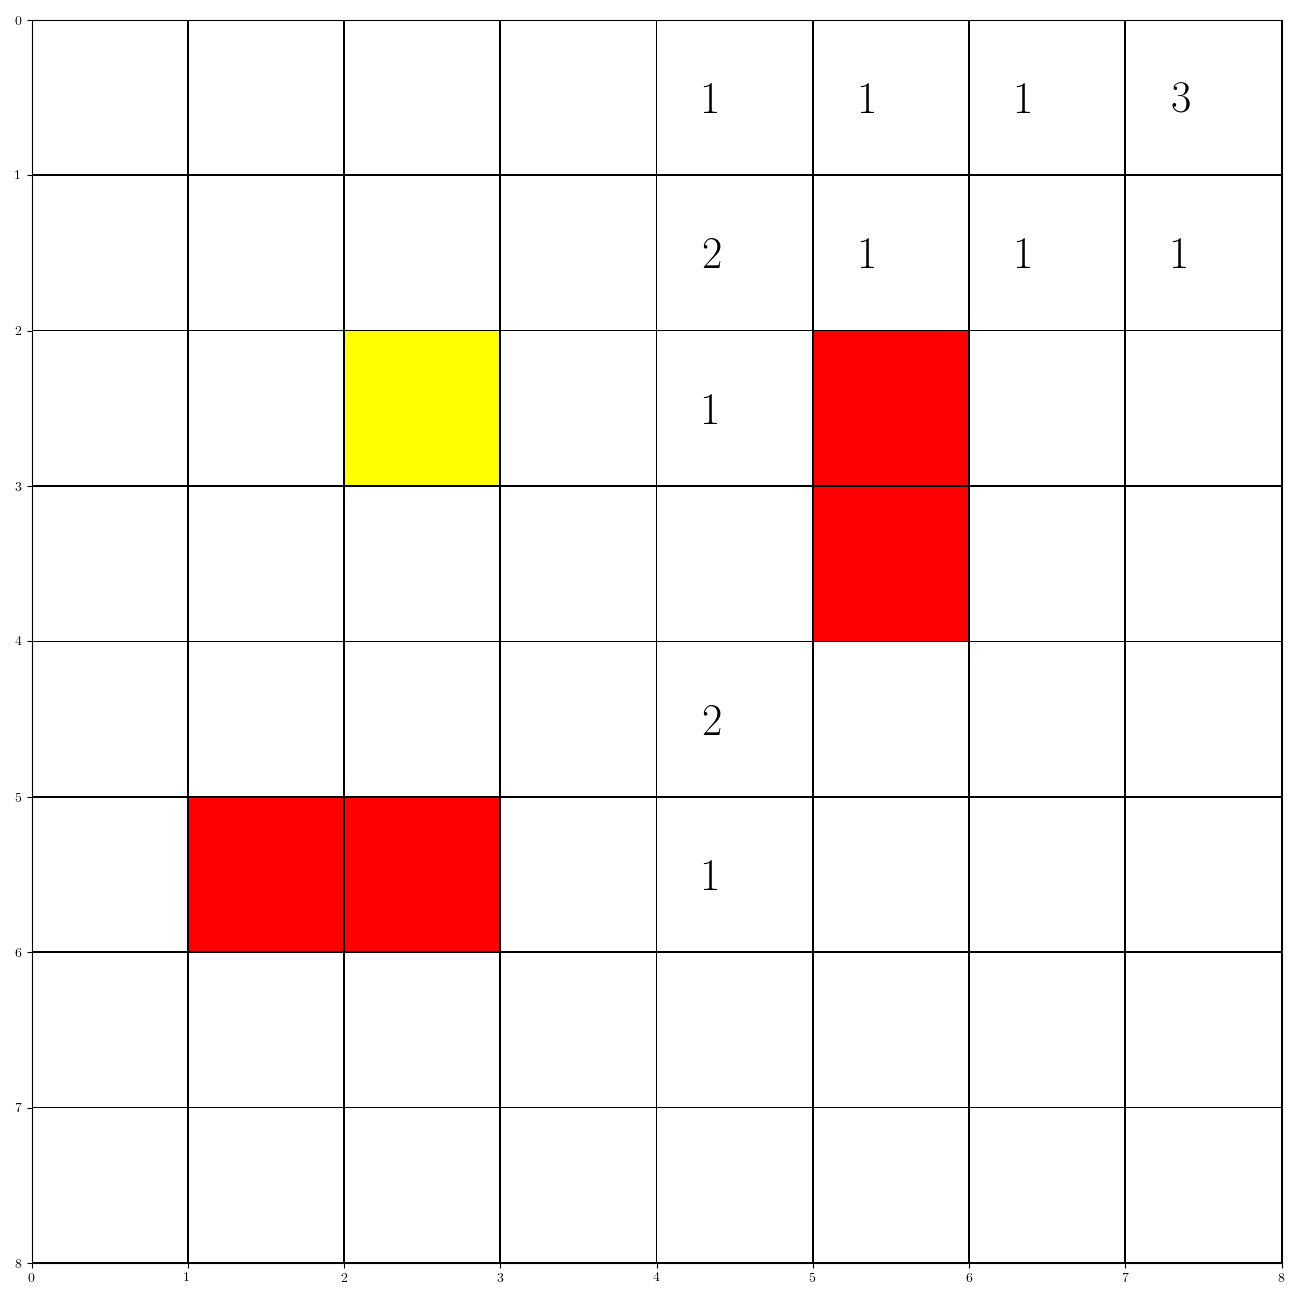
\includegraphics[width=\textwidth]{8x8_sparse_demo}
				\caption{8-by-8 grid world for a single agent.}
				\label{fig:8-by-8_grid_world}
			\end{minipage}
		}
	\end{center}
\end{figure}

\section{32-by-32 Grid World}\label{sec:32by32grid}

\begin{figure}[H]
	\begin{center}
		\fbox{
			\begin{minipage}{1\textwidth}
				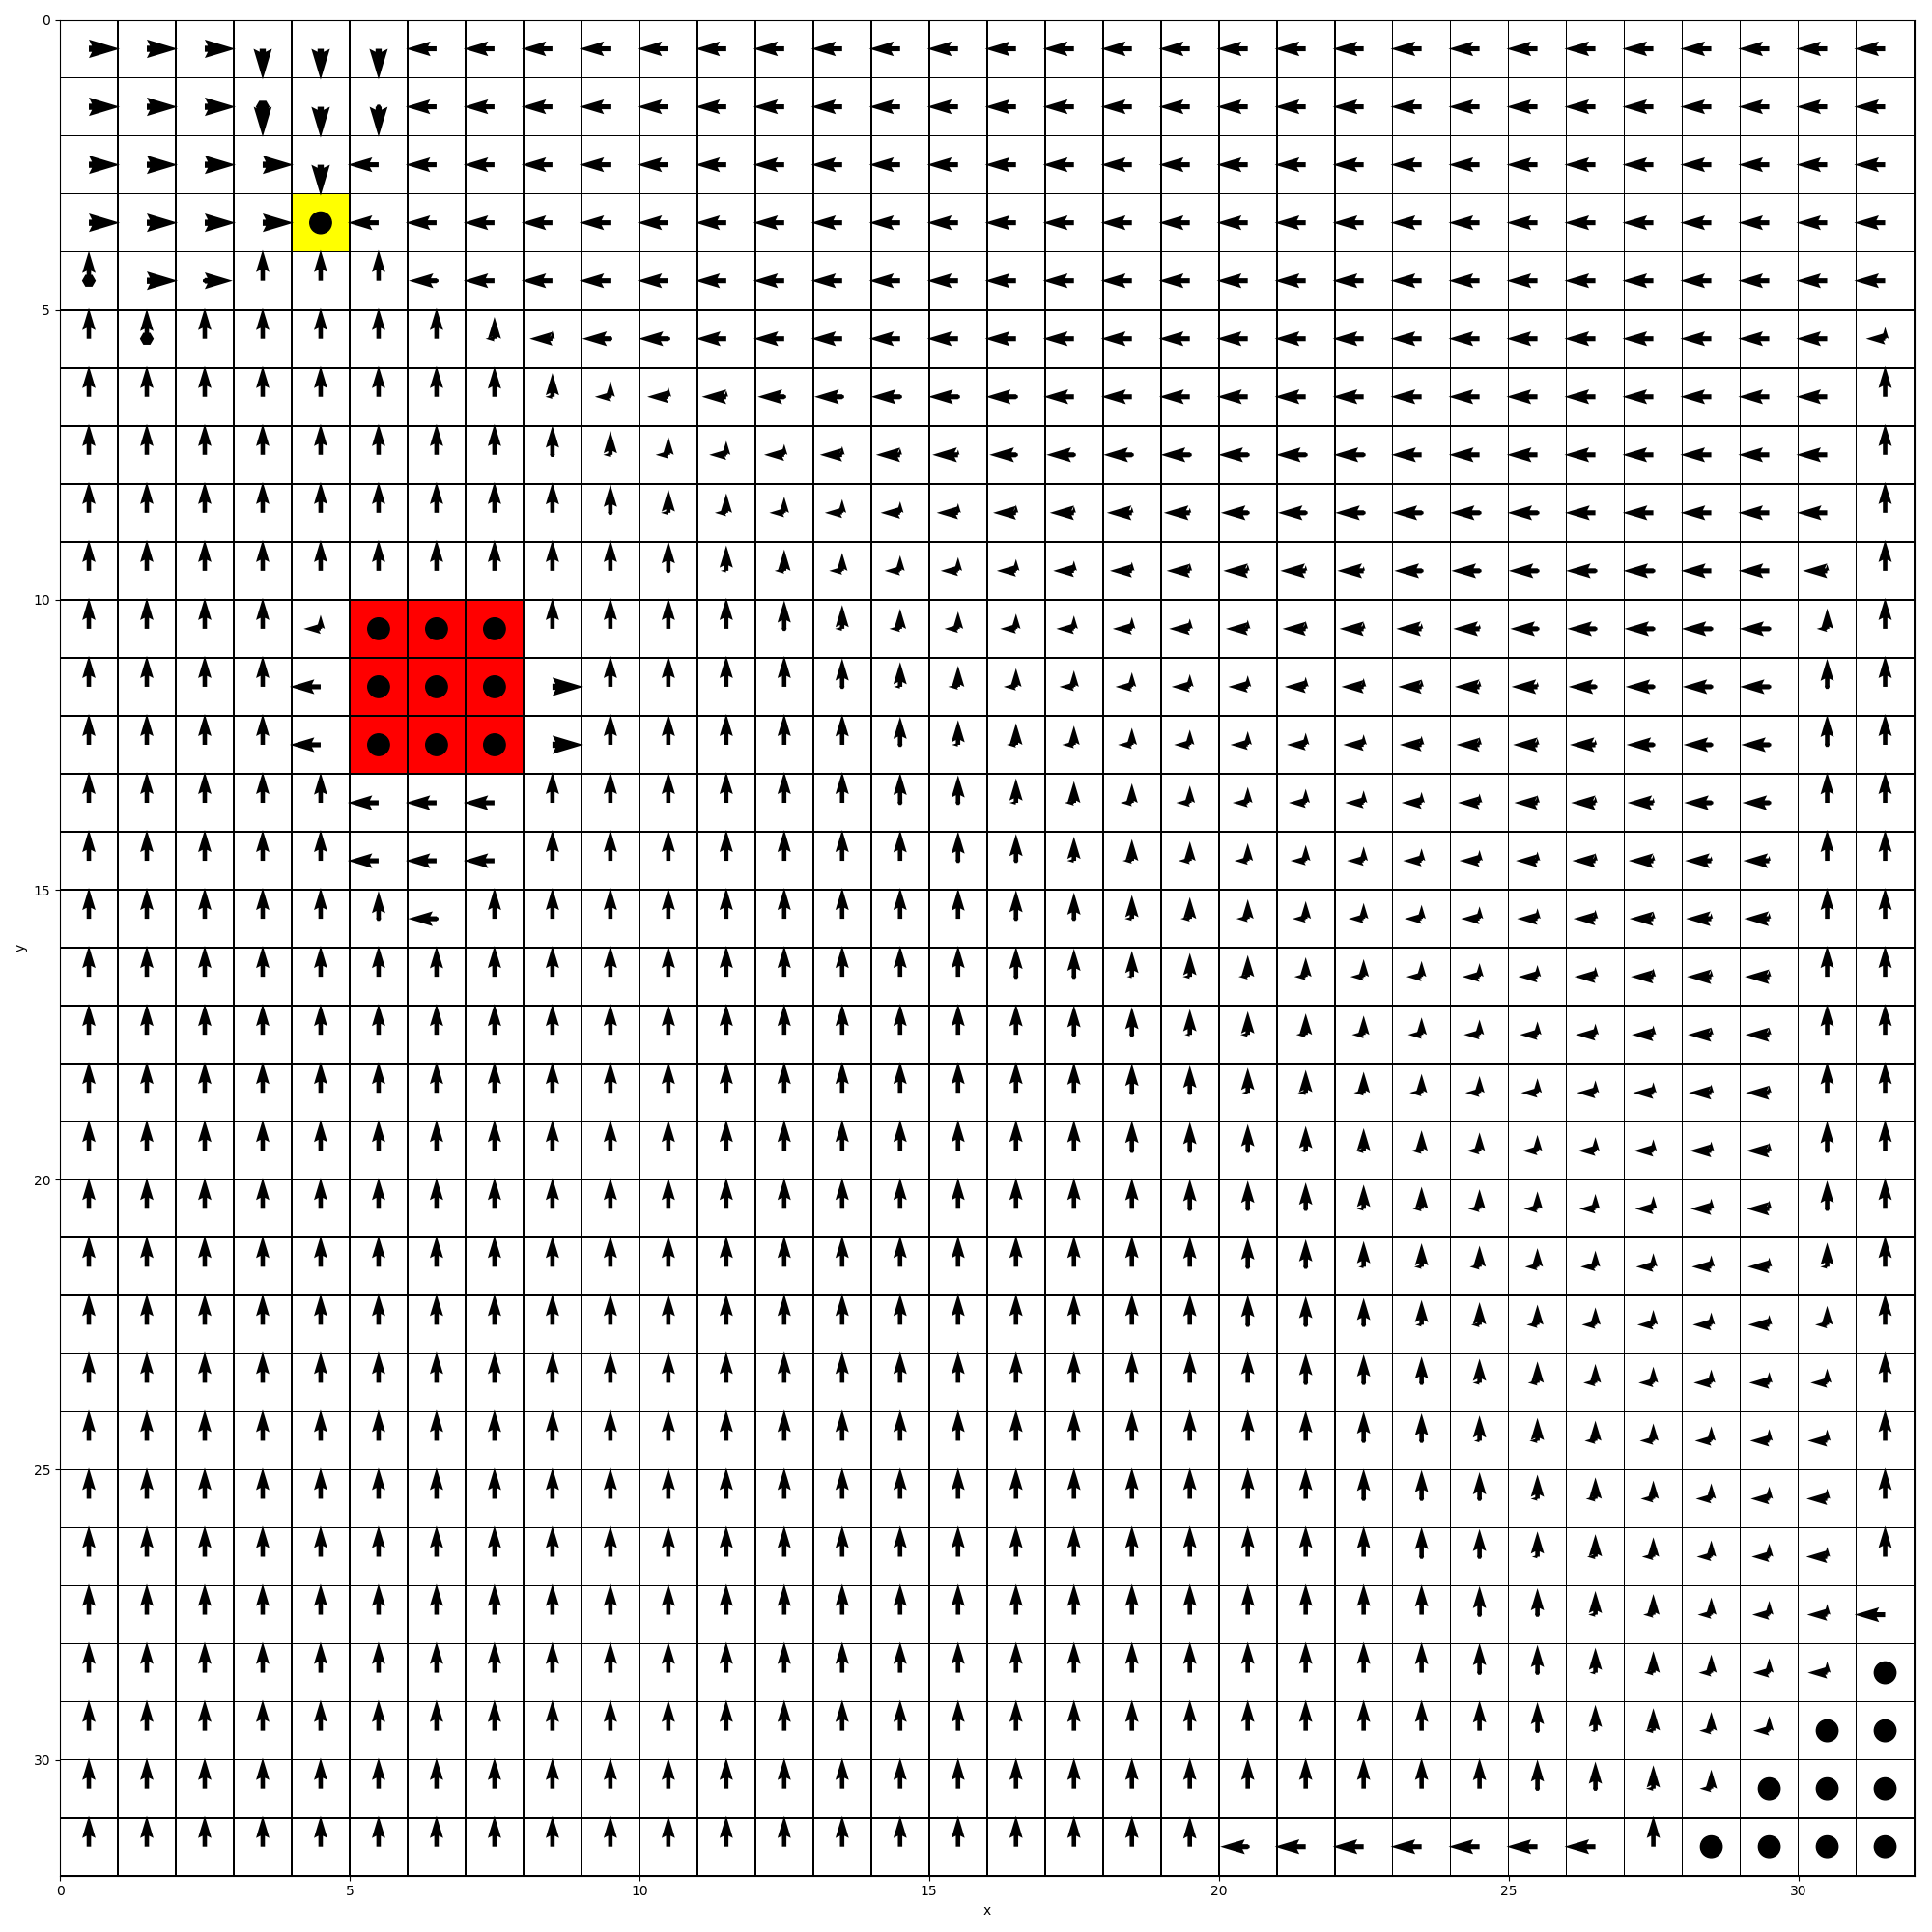
\includegraphics[width=\textwidth]{large_grid_true_policy}
				\caption{True policy of \agent{2} in a single agent environment. Grid size is 32-by-32. Arrow sizes are proportional to probability of taking the action in each direction. Dots represent the stay-action.}
				\label{fig:large_grid_true_policy}
			\end{minipage}
		}
	\end{center}
\end{figure}


\begin{figure}[H]
	\begin{center}
		\fbox{
			\begin{minipage}{1\textwidth}
				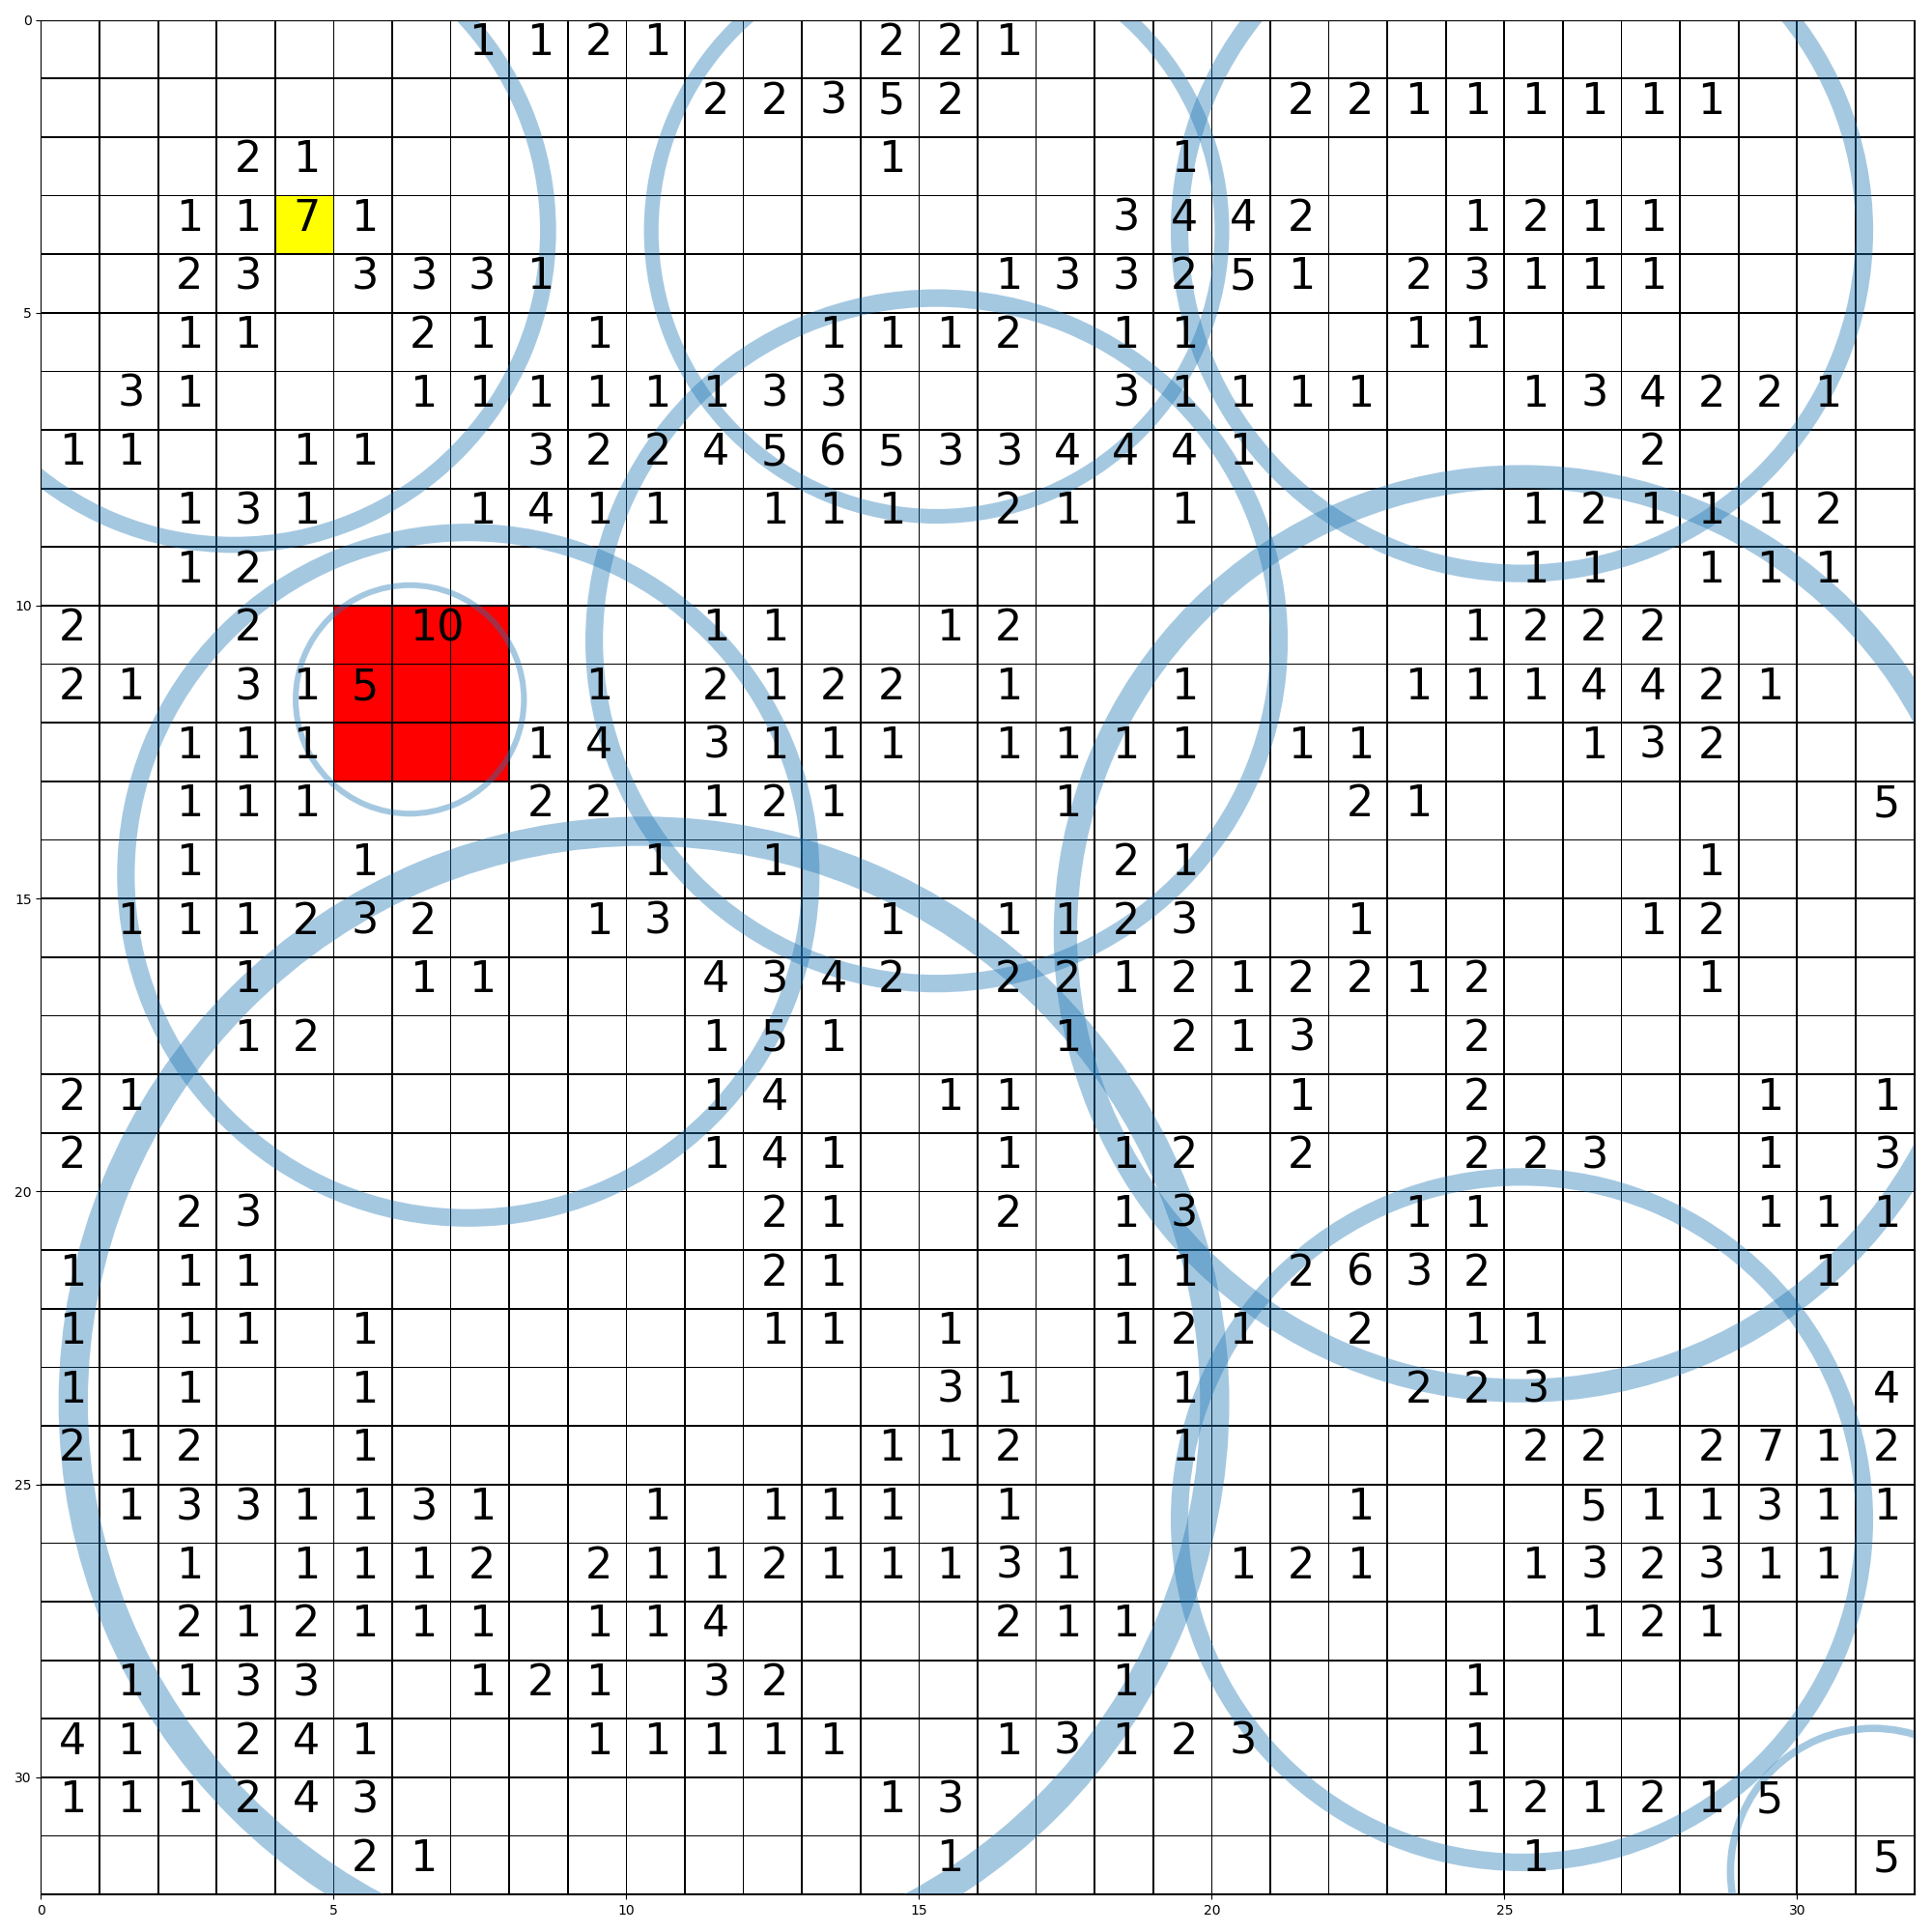
\includegraphics[width=\textwidth]{large_grid_visit_count}
				\caption{Visitation count given 150 trajectories with 5 time steps using the true policy of \agent{2} (Fig. \ref{fig:large_grid_true_policy}) in a single agent environment. Grid size is 32-by-32. Blue circles represent the standard deviation of kernels used.}
				\label{fig:large_grid_visit_count}
			\end{minipage}
		}
	\end{center}
\end{figure}


\begin{figure}[H]
	\begin{center}
		\fbox{
			\begin{minipage}{1\textwidth}
				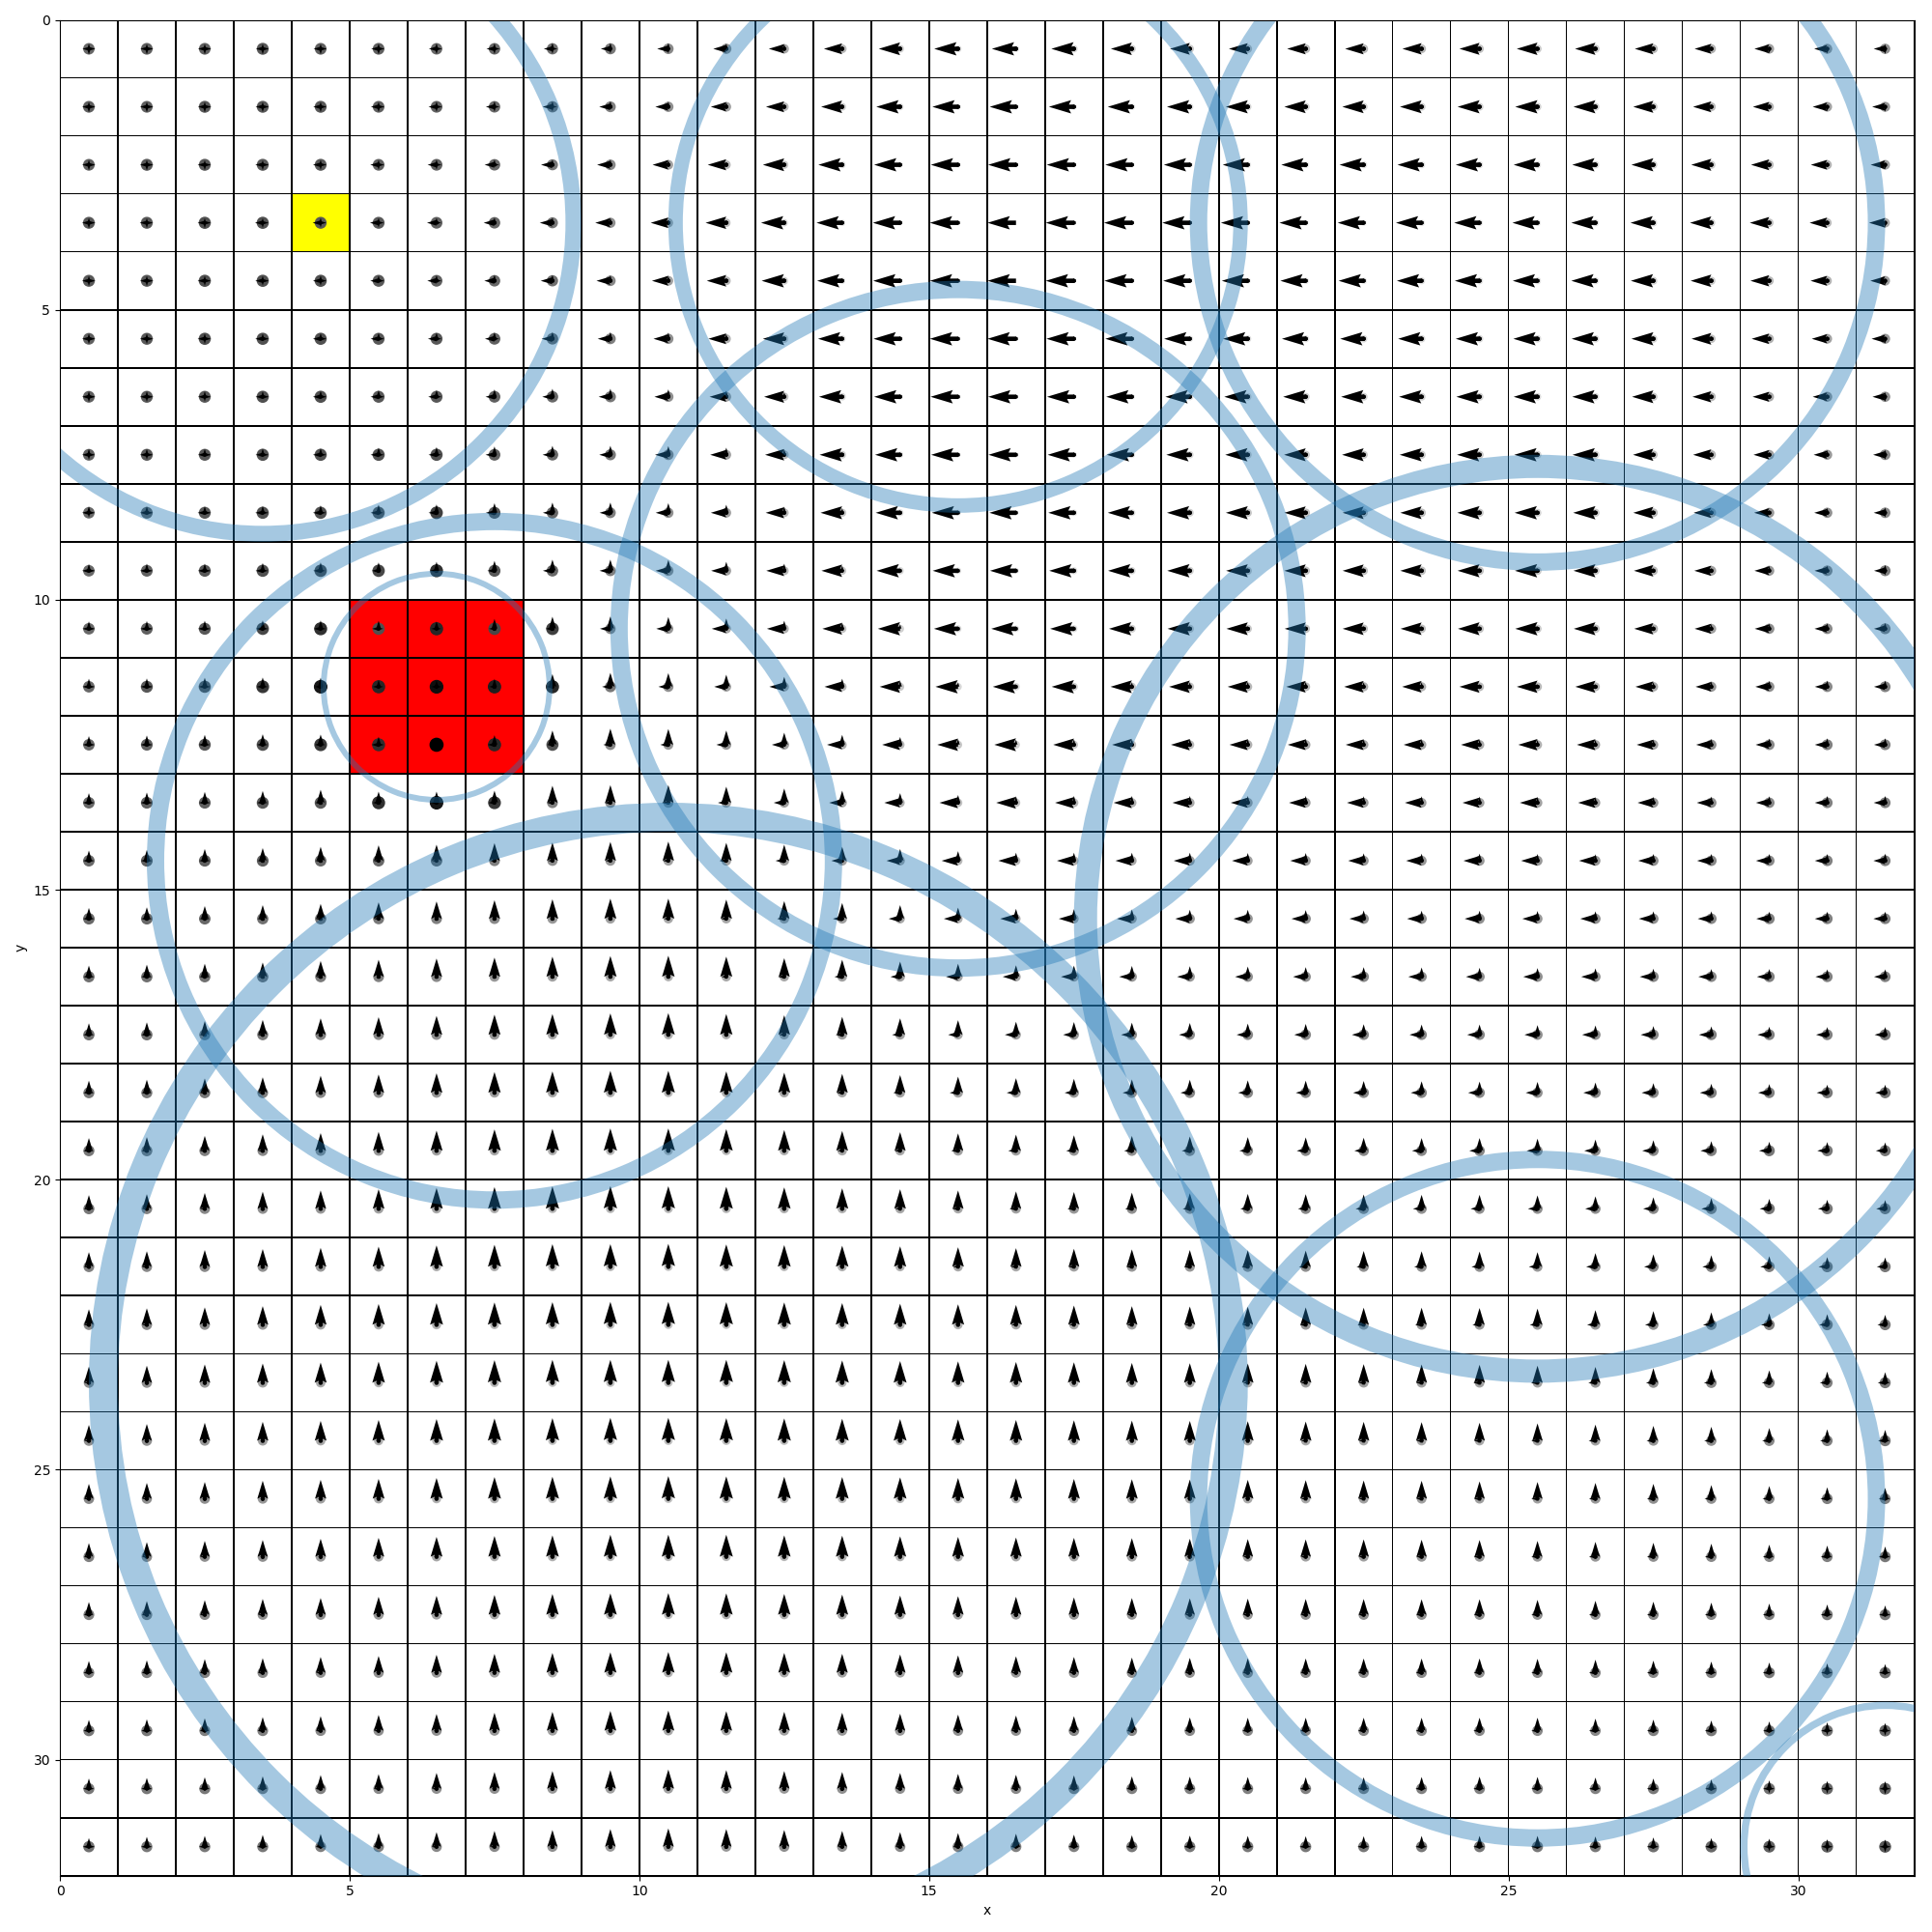
\includegraphics[width=\textwidth]{large_grid_inferred_policy}
				\caption{Inferred policy of \agent{2} in a single agent environment given visitation count (Fig. \ref{fig:large_grid_visit_count}) in a single agent environment. Grid size is 32-by-32. Arrow sizes are proportional to probability of taking the action in each direction.}
				\label{fig:large_grid_inferred_policy}
			\end{minipage}
		}
	\end{center}
\end{figure}


\begin{figure}[H]
	\begin{center}
		\fbox{
			\begin{minipage}{1\textwidth}
				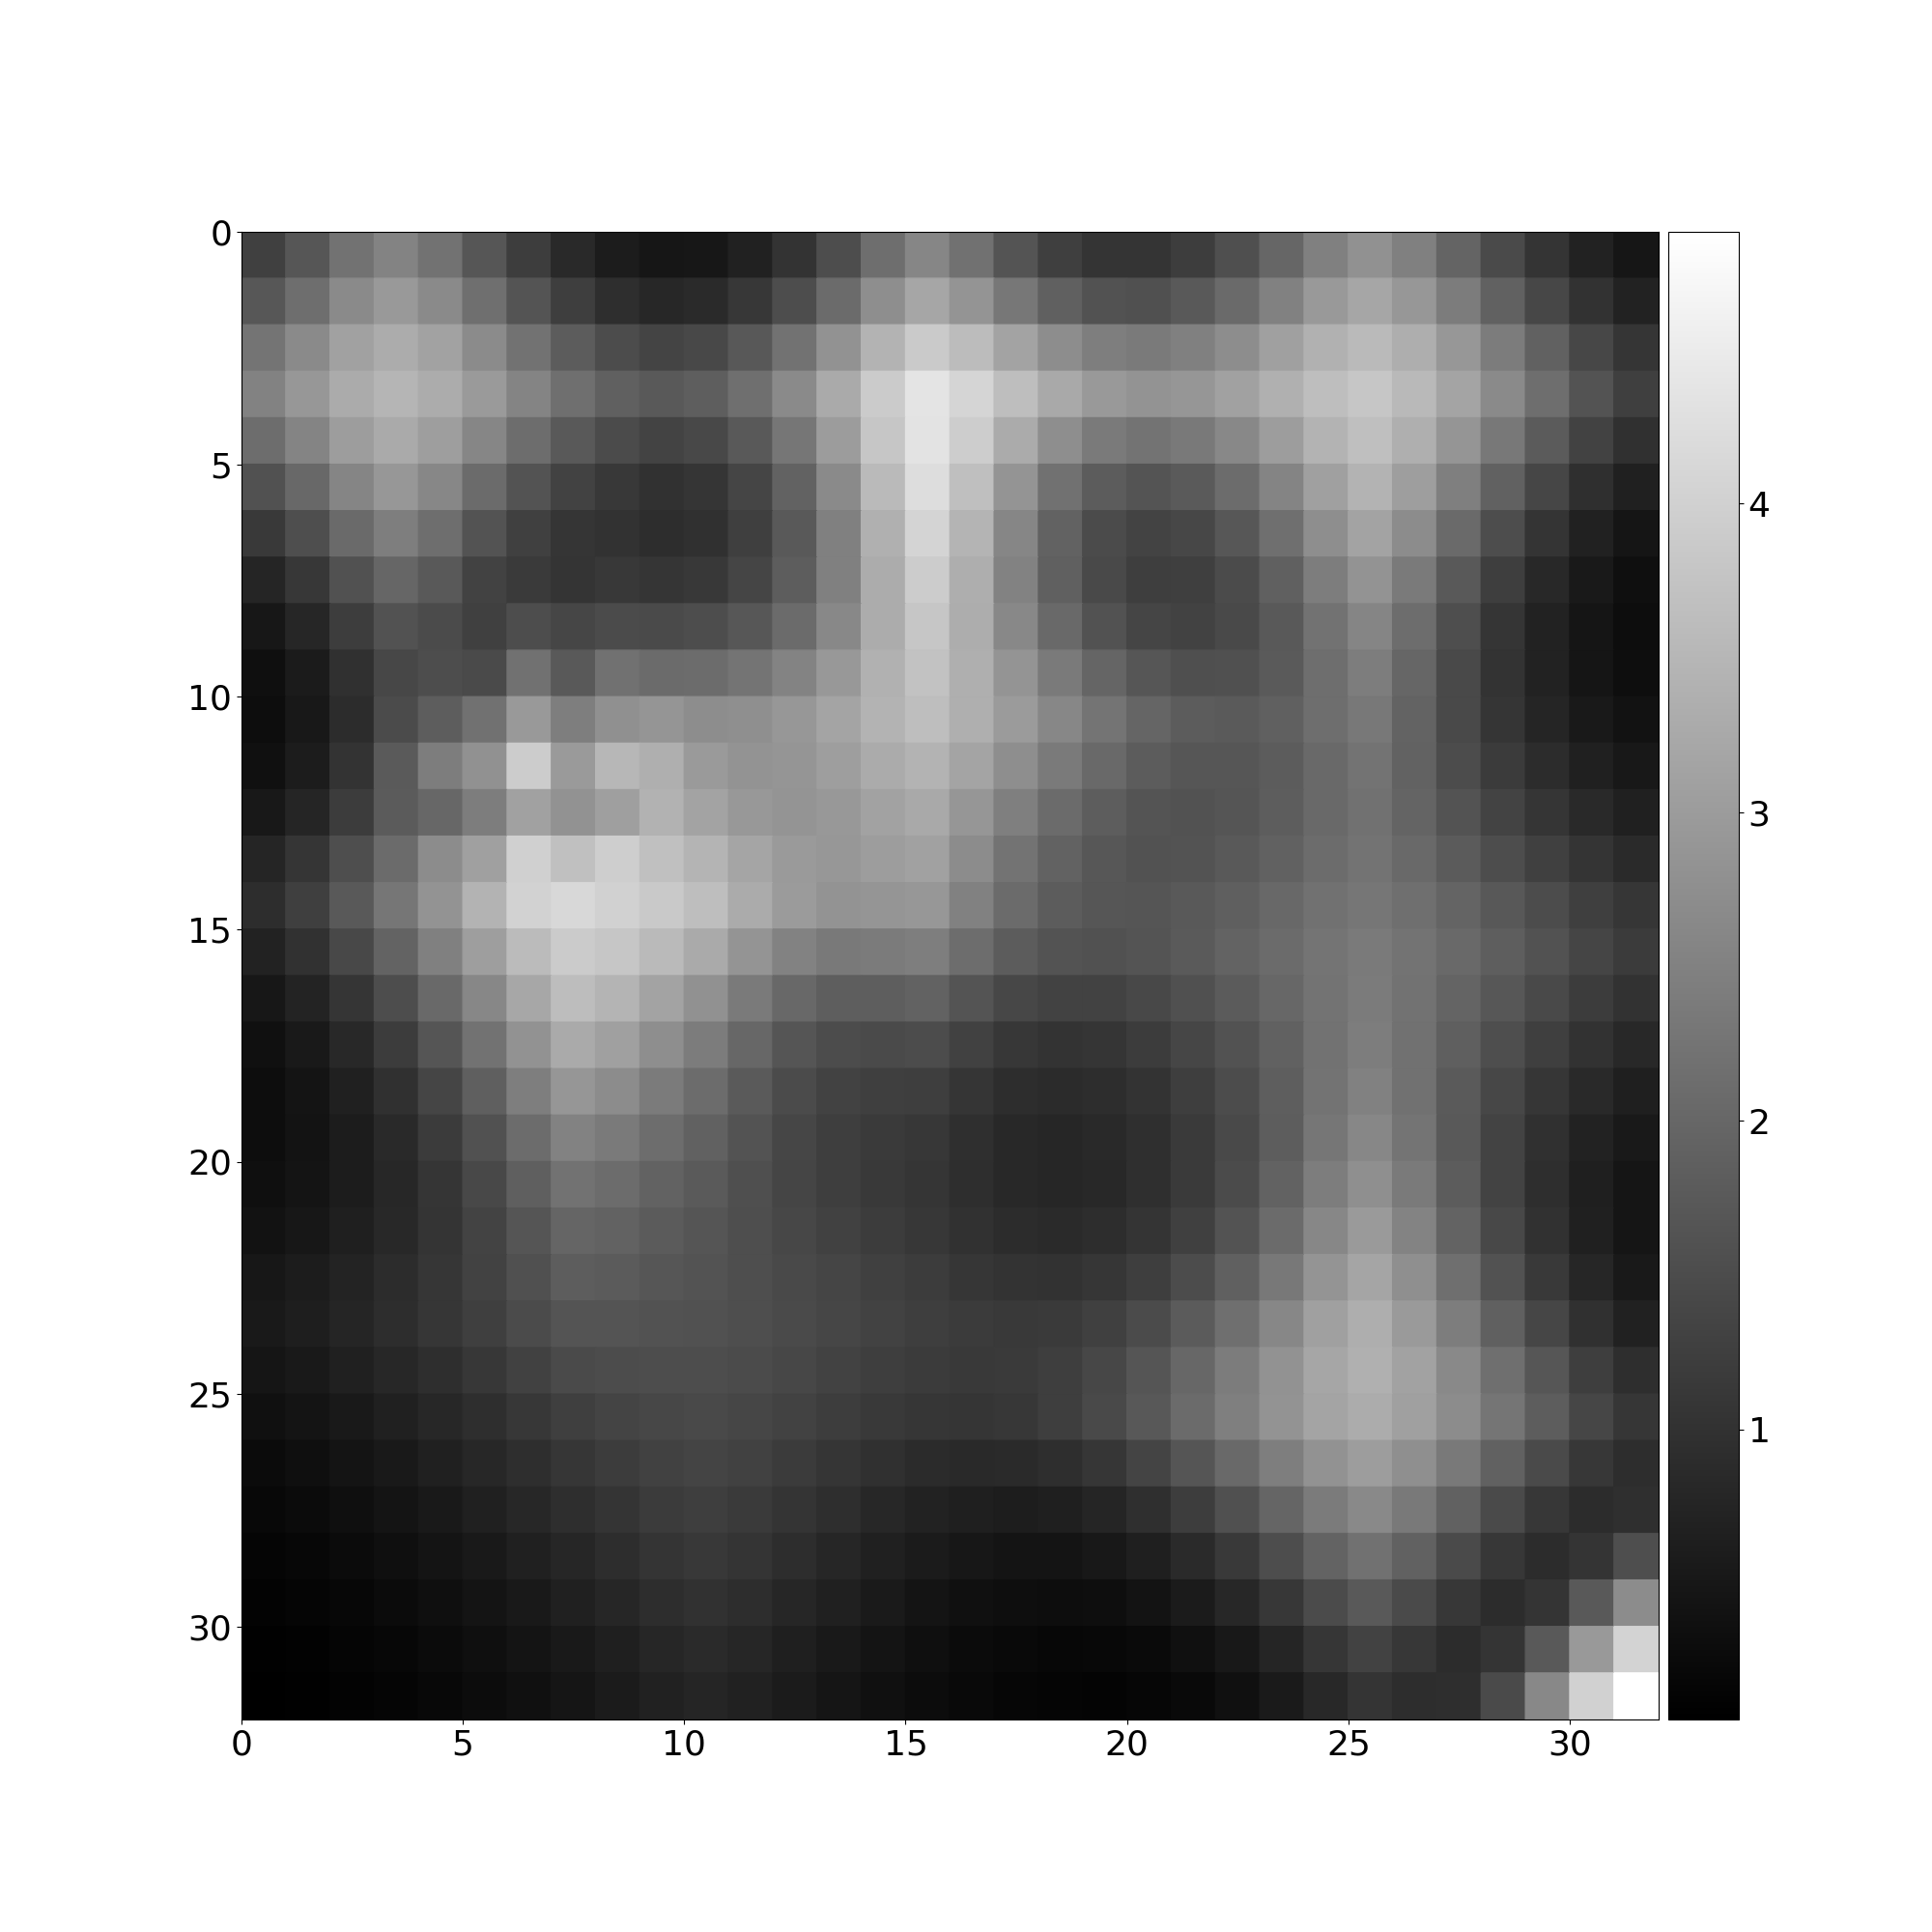
\includegraphics[width=\textwidth]{large_grid_omega}
				\caption{The numerator of Eq. \ref{eq:active_initial_set}, $\sum_{a_2} \Omega(s,a_2)$, is proportional to the probability of initial state being selected after inference results in Fig. \ref{fig:large_grid_inferred_policy}. This heatmap is an alternative visualization of the 3D bar-plot like Fig. \ref{fig:single_agent_uncertainty_surface}}
				\label{fig:large_grid_omega}
			\end{minipage}
		}
	\end{center}
\end{figure}

\begin{figure}[H]
	\begin{center}
		\fbox{
			\begin{minipage}{1\textwidth}
				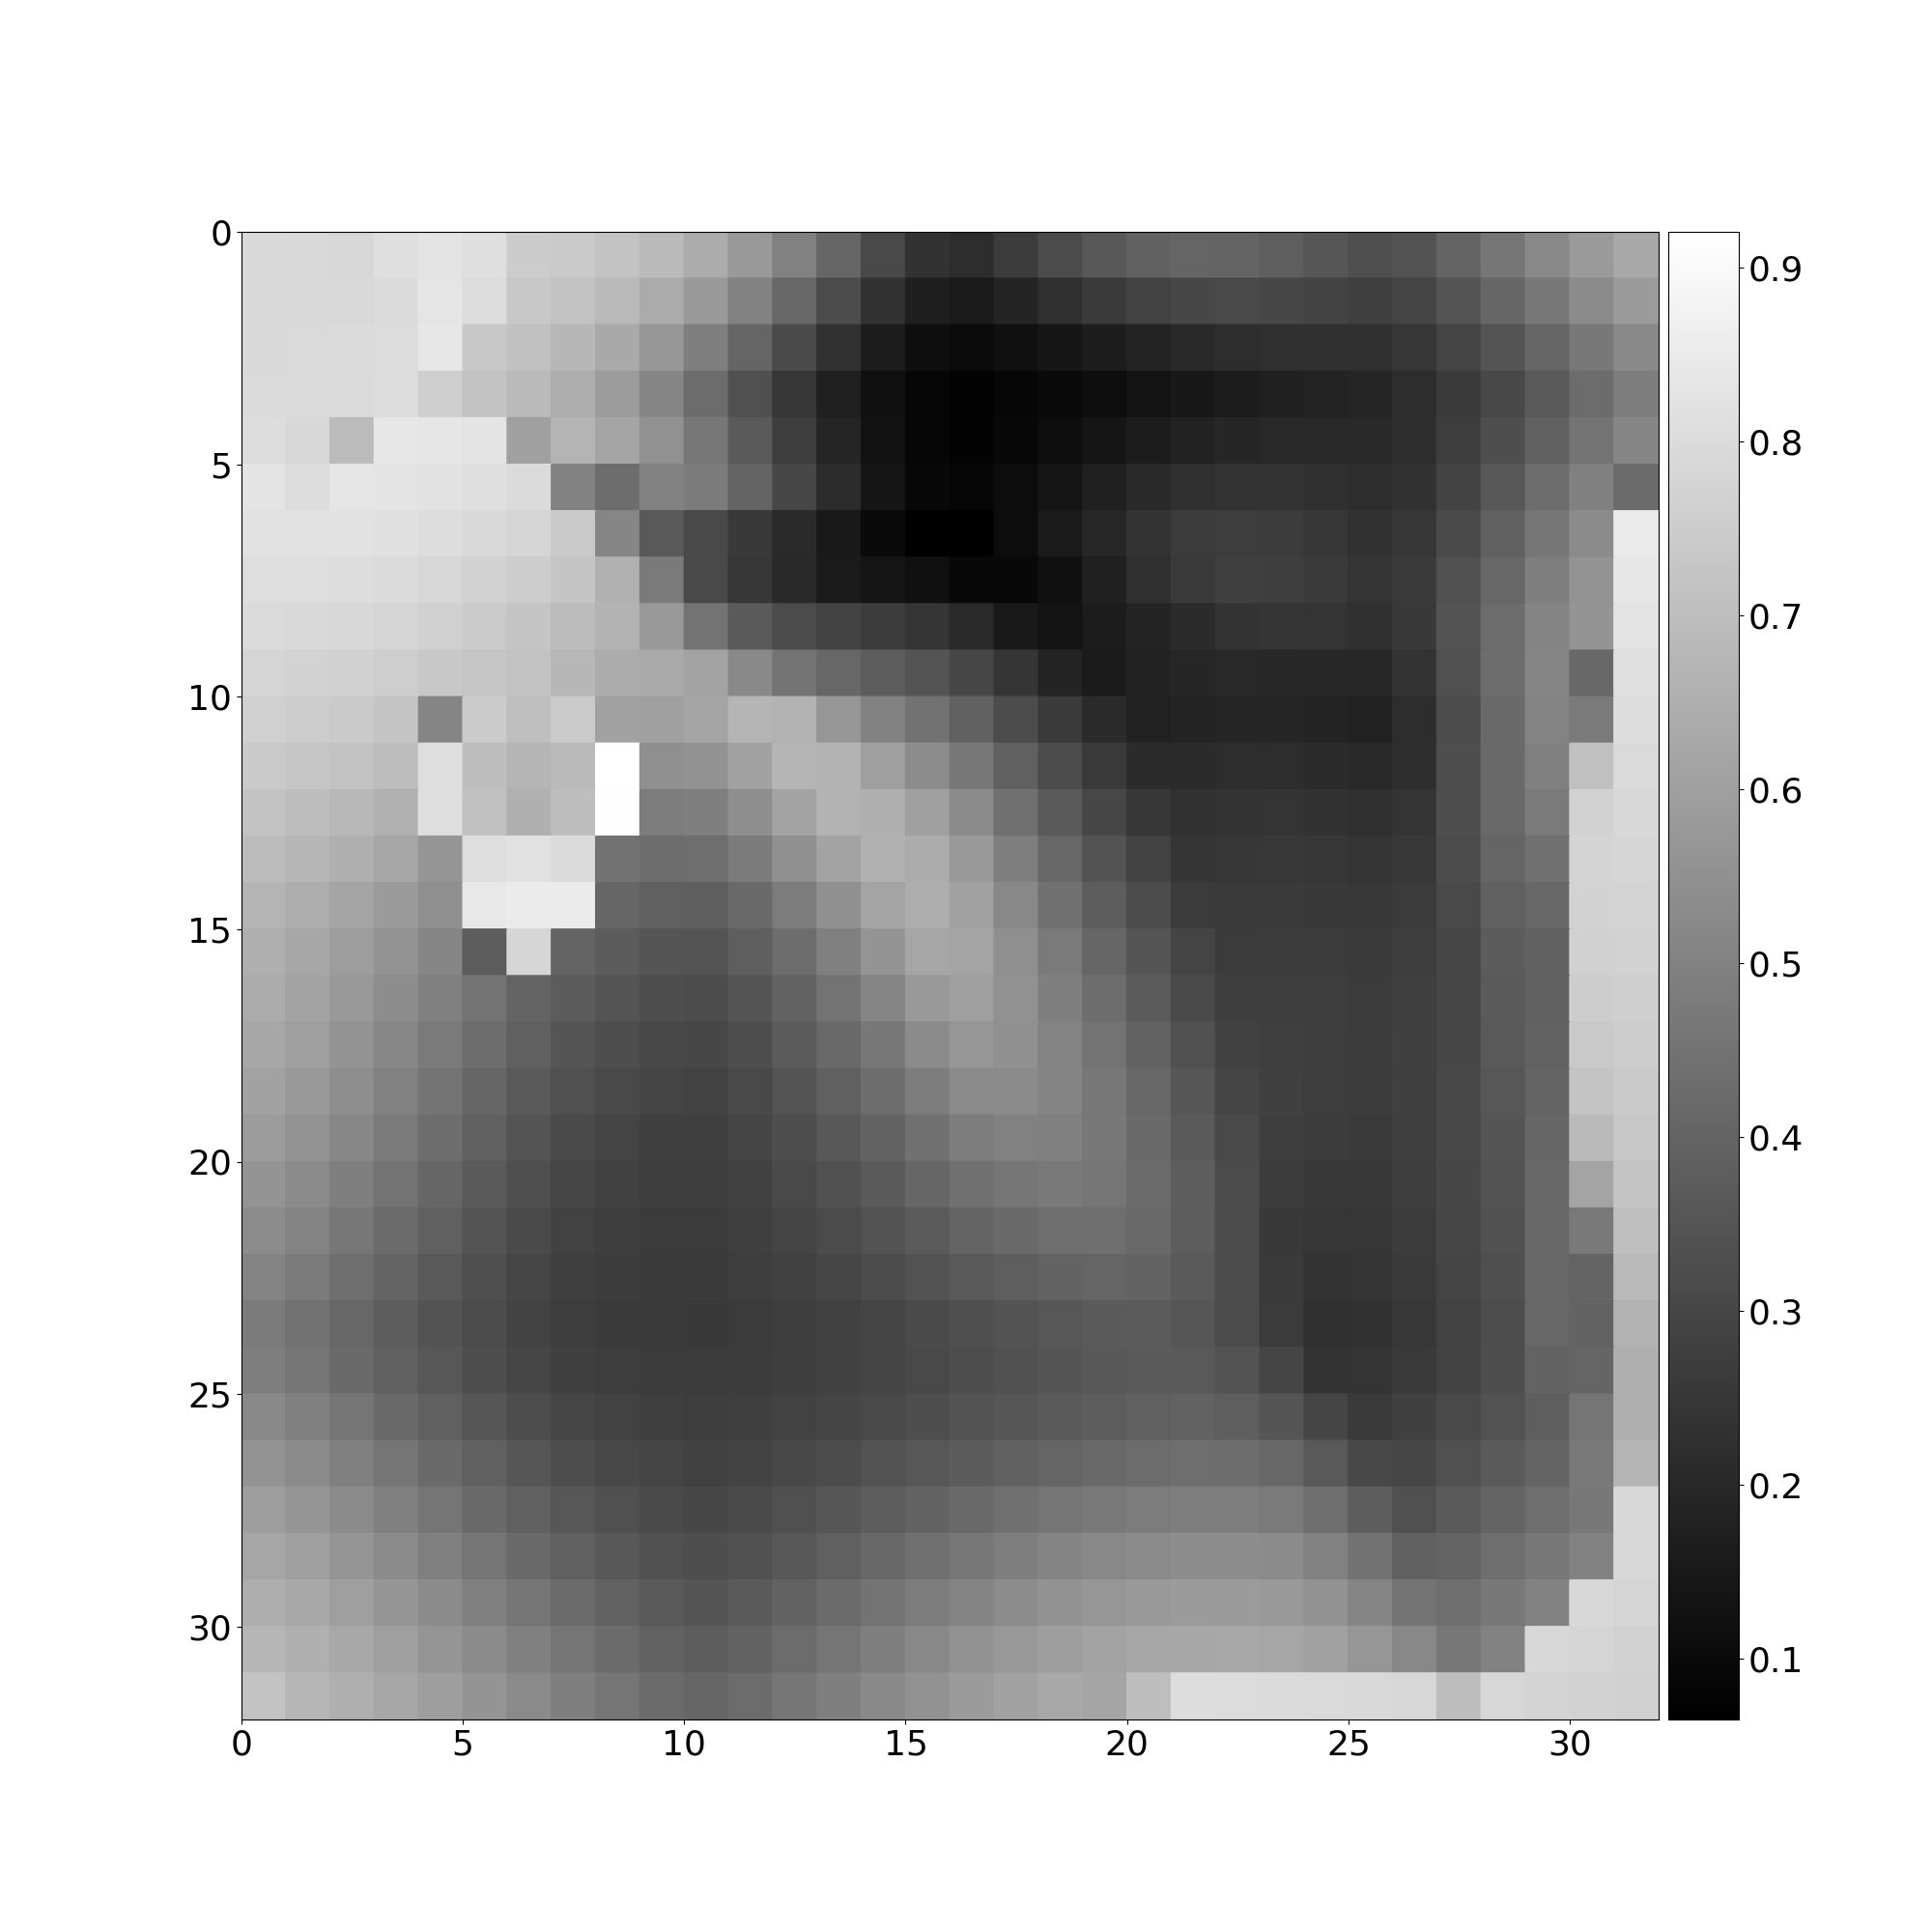
\includegraphics[width=\textwidth]{large_grid_error_magnitude}
				\caption{The true error, \OneNorm{\policy{2},\estimate{\policy{}}_2}, after inference results in Fig. \ref{fig:large_grid_inferred_policy}}
				\label{fig:large_grid_error}
			\end{minipage}
		}
	\end{center}
\end{figure}


%
%\listoftodos
% Last and least (at least, that's what the library says) - the
% Bibliography.


% you can save some space by having the bibliography singlespaced, if you want
\singlespacing

%
% You should become familiar with the BibTeX program, which
% uses a *.bib-file to collect all citations that you have. It's a lot
% prettier than typing all the citations right into the document. The
% reference to citations also works well that way, but the exact
% explanation of that will be on the CS-GSO homepage, whenever I'll ever
% have time for that.
%
%
% If you use BibTeX, the bibliography is very easy. You refer to
% citations in the text with \cite{tag}, where tag is the tag that you
% defined in the bib-file.
% Then, you run bibtex once in a while during compilation, and the
% rest is done in two lines:


\bibliographystyle{alpha}
\bibliography{refs}

% which assumes a file foo.bib in your working directory.
% The word ``Bibliography'' will appear in your document as soon as
% you used ``bibtex'' on the command line.
%
% For reference on this, refer to the CS-GSO homepage.

%============================
%That's all, folks. Have fun.
%
%                     Andreas
%============================


\end{document}
